
\documentclass[french,a4paper]{report}
\usepackage[utf8]{inputenc}
\usepackage{babel}
 \usepackage{graphicx,texhelp,fancyhea,mytitle} 
\usepackage[hidelinks]{hyperref}
 
\parskip=10pt
\parindent=0pt

\begin{document}

\title{NODUS 8.x: Note méthodologique}
\author{Bart Jourquin}
\date{Février 2021}
 
\maketitle
\pagestyle{fancyplain}

\bibliographystyle{plain}
\setheader{{\it Table des matières}}{}{}{}{}{{\it Table des matières}}
\setfooter{\thepage}{}{}{}{}{\thepage}
\pagenumbering{roman}

\tableofcontents

\pagenumbering{arabic}

\setheader{{\it CHAPITRE \thechapter}}{}{}{}{}{{\it CHAPITRE \thechapter}}%
\setfooter{\thepage}{}{}{}{}{\thepage}%

\chapter{Introduction}

\section{What is Nodus?}

Nodus is a GIS-based  software specially designed for  multi-modal freight
transport network modeling.


\section{Content of this document}

Nodus 8.x is not provided with a complete reference or user guide. It is
however important that the user has a good understanding of the methodological
framework the software is based on. This is particularly true for the ``Virtual
Networks'' and the different cost functions they need.

This document is largely inspired by the reference guide  written for Nodus 4.0
(1999). Even if the later versions of the software are very different from
version 4.0, the methodological framework remains essentially unchanged.

\fbox{
\begin{minipage}{\textwidth}
Note, however, that Nodus 7.x maked it possible to define lines and services on 
Virtual Networks. This evolution is not discussed in this document. This
functionality is (temporarily) disabled in Nodus 8.0.
\end{minipage}
}

\chapter{Principes de modélisation}

\section{Introduction}



L'objectif poursuivi lors du développement de NODUS est de proposer une nouvelle
solution aux problèmes posés par les flux de marchandises sur un réseau de
transport multi-modal. Dans cette optique, ce chapitre, qui se présente comme un
court rappel théorique des différents concepts de base de la modélisa\-tion des
réseaux de transport, se limitera essentiellement aux modèles de choix modal et
d'affectation les plus connus, afin de les comparer à ce qui est mis en oeuvre
dans NODUS.. Toutefois, étant donné qu'il est nécessaire d'avoir des matrices
origines-destinations (O-D) avant de pouvoir mettre en oeuvre le choix modal et
l'affectation, quelques méthodes de génération et de distribution sont également
présentées ici, car elles peuvent être utiles dans les applications pratiques
\footnote{Bien que ces matrices sont souvent considérées comme des données
exogènes} qui seront réalisées avec NODUS.


Mais avant de passer aux différents points cités plus hauts, quelques
con\-si\-dé\-ra\-tions générales sur les fonctions de coûts et les comportements
des différents acteurs dans un système de transport vis-à-vis de la demande de
transport trouvent certainement leur place ici, dans la mesure où la (bonne)
définition de ces fonctions et la compréhension du rôle des différents acteurs
sont la clé du succès d'un modèle.



\subsection{Consid\'erations g\'en\'erales sur les fonctions de co\^ut}




La notion de  ``fonction de coût'' sera souvent reprise  dans les différents
chapitres qui composent cette note méthodologique. Or, ces fonctions sont utilisées
dans des contextes parfois fort différents et ne couvrent d'ailleurs pas
toujours les mêmes réalités. De plus, leur linéarité ou leur non-linéarité
seront souvent discutées. Afin de bien clarifier ces concepts, voici une brève
discussion sur les différents types de coûts utilisés.



Il y a tout d'abord les ''fonctions de coûts liées aux arcs d'un réseau''. Il
s'agit là des coûts%
\footnote{Pour ne pas compliquer les choses à ce stade, le terme ``coût`` sera
utilisé pour toute charge monétaire supportée. Il peut donc s'agir par exemple
d'un coût tel que celui qui est supporté par un chauffeur lorsqu'il utilise son
camion} supportés par un usager qui emprunte ce segment du réseau durant un
voyage. Il sera souvent considéré que le coût total de transport est linéaire
avec la distance parcourue et/ou la quantité transportée. Evidemment, et pour
peu qu'il y ait des coûts fixes, le coût moyen de transport sera alors
non-linéaire (Voir figure \ref{f2_1}).

\begin{figure}[htbp]
\centerline{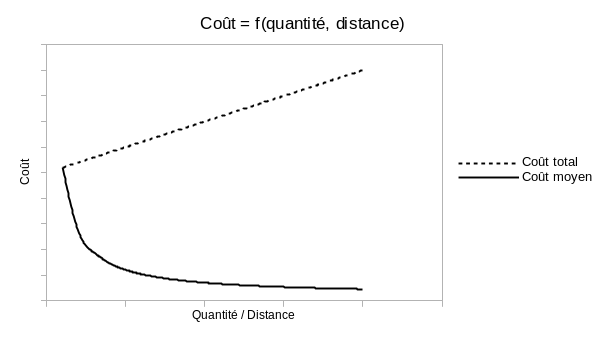
\includegraphics[width=12cm]{f2_1.png}}
\caption{\label{f2_1} Relation entre la quantit\'e/distance et le co\^ut}
\end{figure}


Toutefois, les coûts totaux sur les arcs ne sont pas toujours linéaires par
rapport à la quantité transportée. C'est ainsi que les coûts de manutention ne
sont pas linéaires par rapport à la quantité de marchandises à charger ou
décharger.



Dès le moment où il faut tenir compte des phénomènes de congestion, il  faut
introduire le flux (quantité totale transportée sur un arc déterminé) comme
variable explicative du coût. Le coût total de transport évolue alors de manière
exponentielle par rapport à ce flux, comme illustré dans la figure \ref{f2_2}

\begin{figure}[htbp]
\centerline{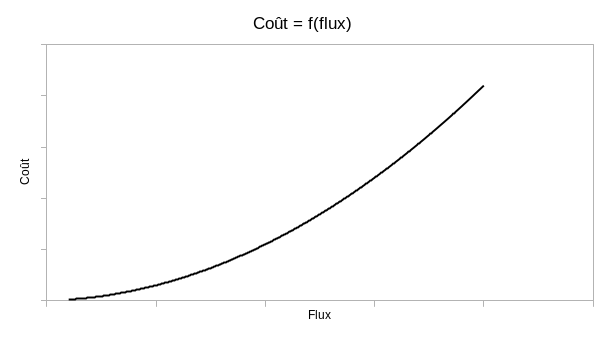
\includegraphics[width=12cm]{f2_2.png}}
\caption{\label{f2_2} Relation Co\^ut-Flux}
\end{figure}


Reste maintenant à considérer le coût total sur le système de transport. Bien
qu'il existe différentes méthodes d'affectation du flux sur un réseau, elles ont
toutes en commun le fait de minimiser une fonction objectif. Ces fonctions
objectif peuvent également prendre différentes formes. C'est ainsi qu'en se
plaçant du point de vue de la collectivité, il s'agit de minimiser le coût total
de transport sur le système. Par contre, il faudra minimiser le coût moyen des
voyages s'il s'agit du point de vue de l'usager.

D'une manière générale, lorsque les fonctions de coût de transport sont
linéaires par rapport aux quantités, et que la congestion ne doit pas être
modélisée, en sorte qu'il est toujours possible d'affecter les transports en
choisissant la solution (choix d'un mode, d'un moyen ou d'une route) de coût
minimum par la mise en oeuvre d'un bon algorithme de recherche de chemin sur un
graphe, il n'y a pas à proprement parler de fonction objectif dans la mesure où
il y a discontinuité entre les différentes solutions possibles. Cependant, si
les coûts des différentes combinaisons convexes des solutions de répartition des
quantités sont distingués, la fonction de coût obtenue serait une fonction
linéaire (non strictement convexe), car toutes les fonctions de coûts sur les
différents segments sont linéaires par rapport aux quantités transportées sur ce
segment.

Par contre, lorsque des fonctions de coût non linéaires (convexes)
sont utilisées sur les arcs, ce qui doit être le cas pour les
modèles qui tiennent compte du niveau de congestion sur le réseau,
les solutions ne seront en général pas du type ``tout ou rien``,
mais il y aura une répartition des quantités entre les différents
modes, moyens et routes disponibles. L'ensemble de ces solutions
potentielles forme alors une fonction de coût total continue
convexe résultant de la sommation des différentes fonctions
convexes.



Il y a plusieurs concepts de coûts à prendre en considération et c'est la raison
pour laquelle, tout au long de ce texte, il sera bien précisé ce à quoi les
coûts utilisés font référence.



\subsection{Le comportement des acteurs sur un syst\`eme de transport}

Les étapes de génération et de distribution du modèle classique à
quatre étages sont des approches plutôt agrégées de la décision de
transport. Ce n'est qu'au moment où il faut réellement se pencher
sur le choix d'un mode de transport et sur le choix d'une route à
emprunter sur un réseau que les comportements des acteurs dans le
système de transport sont analysés plus en profondeur, sous un
angle plus pointu.

Classiquement, les acteurs considérés sont les producteurs de biens (qui jouent
le rôle d'expéditeur), les consommateurs et les transporteurs. Les producteurs
et les consommateurs ne sont pas localisés au même endroit. L'analyse des
mécanismes qui régissent les liens entre ces différents acteurs est la raison
même de l'existence de l'économie des transports et de tous les outils
informatiques, tels que NODUS, qui ont été développés ces dernières années.


Les expéditeurs sont l'ensemble des agents économiques qui prennent la décision
d'affecter et de distribuer un certain flux de marchandises entre une origine et
un certain nombre de destinations. Les transporteurs représentent en réalité un
ensemble de différentes entités impliquées dans la décision de transport. On y
trouve par exemple les département ``expéditions``, ``distribution`` ou
``réception`` des firmes. La décision de transport peut être quelque chose de
complexe, mais comme le dit si bien Roberts \footnote{Roberts, P.O., 1976,
``Forecasting Freight Flows Using a Disaggregated Freight Demand Model``, CTS
Report 76-1, Center for Transportation Studies, MIT.},``la seule motivation qui
pousse au déplacement de la marchandise est la raison économique``. Dès lors, la
décision du transporteur dépend du comportement de l'offre et de la demande et
des prix (de la marchan\-dise) sur le marché.

Lorsque l'expéditeur prend sa décision de transport, il choisit un
transporteur pour effectuer le transport. En économie des
transports, le transporteur est toujours perçu comme un agent
économique qui produit du transport en essayant de maximiser son
profit.

La relation entre les expéditeurs et les transporteurs est
assimilée à celle qui peut exister entre un consommateur et un
producteur de services. Par sa décision d'attribuer un chargement à
un transporteur, l'expéditeur crée une demande pour l'output
produit par ce transporteur. De son côté, le transporteur va
demander un certain prix pour effectuer le transport et crée de ce
fait un certain niveau de service.

Si on ajoute à cela le rôle joué par l'état, on peut représenter les relations
existantes entre les différents acteurs de la manière présentée dans la figure
\ref{f2_3}:

\begin{figure}[htbp]
\centerline{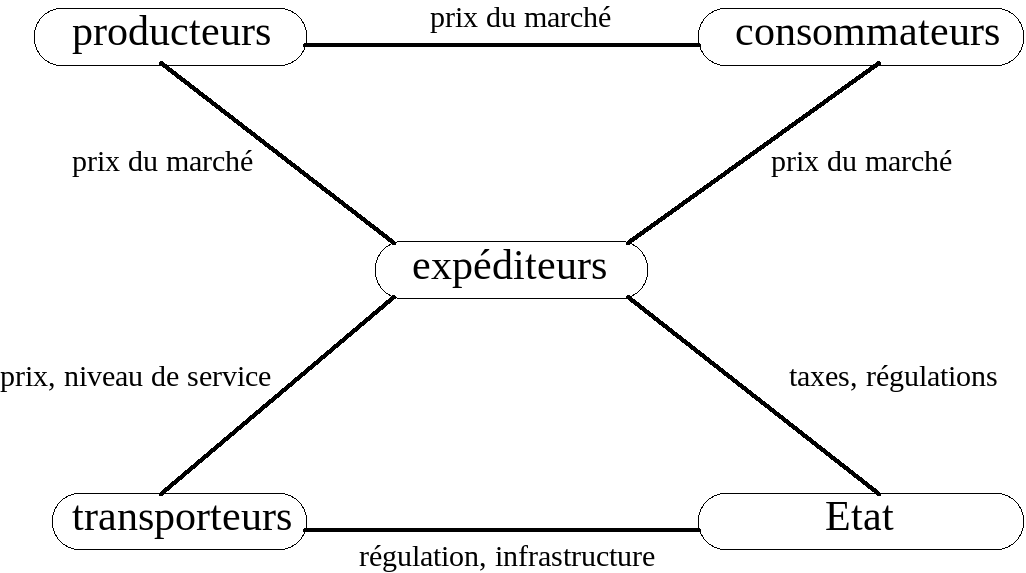
\includegraphics[width=10cm]{f2_3.png}}
\caption{\label{f2_3} Les acteurs d'un syst\`eme de transport}
\end{figure}


Il reste néanmoins évident que toutes ces interactions ne peuvent
exister que dans la mesure où il existe une demande pour le
transport. Cette dernière est fonction de différents facteurs
explicatifs parmi lesquels:

\begin{itemize}

\item Le prix du service de transport: comme la demande de n'importe quel
bien, la demande de transport est en principe une relation
décroissante du prix du transport.

\item Le prix des autres modes de transport: alors que certaines catégories
de marchandises sont transportées (presque) uniquement par un seul
mode de transport, certaines catégories peuvent voyager par des
modes différents. Une variation du prix sur un mode de transport
peut de ce fait influencer la demande pour un autre mode.

\item Le prix des biens complémentaires: on peut considérer le transport comme
faisant partie d'un processus de production. Un exemple classique
est celui de la production d'énergie électrique par des centrales
thermiques qui doivent faire venir le combustible (charbon, fuel)
par péniche ou par camion. Il est évident que la demande de
transport pour le combustible est directement fonction du niveau de
production d'énergie.

\item La durée: le transport est un bien extrêmement particulier dans la mesure
où son utilisateur est ``impliqué`` dans la production du service de transport
par le temps que la marchandise passe à se déplacer. La durée du transport joue
un rôle capital pour expliquer la demande de transport et le choix modal. La
demande de transport est en relation inverse avec la durée nécessaire au
transport. L'élasticité-temps est donc négative. La demande de transport est
également sensible à la vitesse, mais cette dernière apparaît davantage comme un
élément déterminant la durée du transport que comme un facteur explicatif
supplémentaire.

\item La liberté de disposition: les expéditeurs sont très sensibles à ce
facteur, qui explique en partie le succès du transport routier.

\item La capacité: l'adéquation entre les caractéristiques des marchandises à
transporter (volume, poids) et celles du mode de transport détermine souvent le
choix du mode.

\item La sécurité et le respect des délais. les transports de marchandises
sont sensibles aux risques encourus (bien que la perception de ce
risque est souvent subjective) et au respect des délais
d'exécution.

\end{itemize}



\section{Techniques de g\'en\'eration et de distribution}

Cette section présente quelques techniques de
base qui concernent la génération et la distribution\footnote{Le lecteur
intéressé par une présentation plus approfondie de ces techniques lira avec
intérêt le livre de J. de D. Ortuzar et L. G. Willumsen, ``Modelling
Transport``, Wiley, 2011.}. Pour rappel, NODUS ne contient pas de modules de
génération et de distribution: les matrices O-D doivent donc toujours être
fournies, et les quelques paragraphes qui suivent doivent être considérés comme
une petite présentation théorique, utile lorsque des matrices O-D ne sont pas
disponibles ou lorsqu'elles sont partielles ou anciennes. La génération permet
en effet d'estimer les flux totaux en provenance et à destination des
différentes zones du réseau tandis que la distribution permet de créer une
matrice O-D à partir de ces flux totaux.

Encore une fois, les pages qui suivent n'ont aucunement la prétention de
présenter un état complet de l'art en la matière, l'objectif étant simplement
ici d'aider le lecteur non familiarisé avec les techniques de base de la
modélisation classique.

\subsection{G\'en\'eration}

L'étape de génération essaye de déterminer l'attraction et l'émission globale de
chaque zone de l'aire géographique étudiée. A ce stade, les liens qui peuvent
exister entre une origine et une destination particulière ne sont pas encore
pris en considération. Les mouvements qui vont et viennent d'un noeud déterminé
sont estimés en classant les flux par catégorie (objectif, période, type de
marchandise, ...) et en déterminant les facteurs qui influencent ces flux. Dans
le cas du transport de marchandises, les critères suivants sont généralement
pris en considé\-ration :

\begin{itemize}
\item la nature des marchandises,
\item la population,
\item le niveau de revenus,
\item nombre d'employés dans les entreprises,
\item le nombre de transactions réalisées,
\item la zone d'influence des firmes,
\item etc.
\end{itemize}

Ces données sont ensuite essentiellement exploitées par:

\begin{itemize}
\item des analyses de régression,
\item des techniques de classification croisées,
\item des techniques de prévision sur les variables utilisées,
\item des techniques de test de stabilité des résultats obtenus.
\end{itemize}

\subsection{Distribution}

L'étape suivante consiste logiquement à distribuer les flux totaux
entre les différents pôles mis en évidence dans l'étape de
génération. En d'autres termes, il s'agit maintenant d'estimer une
matrice O-D.

La littérature présente plusieurs méthodes dont les plus classiques sont les
méthodes du taux de croissance et les méthodes synthétiques.

\subsubsection{Les méthodes du taux de croissance.}

Ces méthodes se basent sur l'existence préalable d'une première
matrice O-D (t). L'utilisation d'un taux de croissance attendu
permet alors d'estimer une nouvelle matrice.

La méthode de base est utilisée seulement d'un taux de croissance
général est disponible  $\tau$. On applique alors $T_{ij} = \tau
t_{ij}$ pour chaque paire ij.

Si un taux de croissance spécifique est disponible pour chaque
origine ou chaque destination $\tau_i$ ou $\tau_j$, on parle de la
méthode du taux de croissance à une seule contrainte.

Dans ce cas, $T_{ij} = \tau_it_{ij}$ pour un taux de croissance
"origine" et $T_{ij} = \tau _jt_{ij}$ pour un taux de croissance
"destination".

Par exemple (voir tableau \ref{tab2_1}), avec une information prévisionnelle de
flux sur les origines (cibles).

\begin{table}[htbp]
\begin{center}
\begin{tabular}{rrrrrrr}
\hline
i$\backslash$j & 1 & 2 & 3 & 4 & $\sum\limits_{i}$ & Cibles $O_i$\\
\hline
1 & 5 & 50 & 100 & 200 & 355 & 400\\ 2 & 50 & 5 & 100 & 300 & 455 & 460\\

3 & 50 & 100 & 5 & 100 & 255 & 400\\ 4 & 100 & 200 & 250 & 20 & 570 & 702\\
$\sum\limits_{i}$ & 205 & 355 & 455 & 620 & 1635 & 1962\\
\hline
\end{tabular}
\caption{\label{tab2_1} Pr\'evision aux origines et destinations}
\end{center}
\end{table}


Le problème peut facilement être résolu en multipliant chaque ligne par le ratio
$O_i/\sum\limits_jt_{ij}$ , qui représente un taux de croissance (voir tableau
\ref{tab2_2}).

\begin{table}[htbp]
\begin{center}
\begin{tabular}{rrrrrrr}
\hline
i$\backslash$j & 1 & 2 & 3 & 4 & $\sum\limits_{i}$ & Cibles $O_i$\\
\hline
1 & 5.6 & 56.3 & 112.7 & 225.4 & 400 & 400\\

2 & 50.5 & 5.1 & 101.1 & 303.3 & 460 & 460\\

3 & 78.4 & 156.9 & 7.8 & 156.9 & 400 & 400\\

4 & 123.2 & 246.3 & 307.9 & 24.6 & 702 & 702\\

$\sum\limits_{i}$ & 257.7 & 464.3 & 529.5 & 701.2 & 1962 & 1962\\
\hline
\end{tabular}
\caption{\label{tab2_2} Application du ratio de croissance}
\end{center}
\end{table}



La méthode du taux de croissance à double contrainte est appliquée lorsque des
estimations sur le nombre futur de mouvements aux origines et aux destinations
sont disponibles. On dispose dans ce cas, pour chaque noeud, d'un facteur de
croissance d'attraction $\tau_i$ et de génération $\Gamma_j$. L'utilisation d'un
facteur moyen $F_{ij}=0.5(\tau_i+\Gamma_j)$ n'est qu'un compromis très
approximatif. Pour résoudre ce problème, on a recours à des processus itératifs,
dont le plus connu est celui de Furness
\footnote{ Furness K. P., 1965, ``Time Function Iteration``,
Traffic Engineering and Control, 7(7), 458-60} qui introduit la
notion de ``facteurs de balancement`` $A_i$ et $B_j$.

\begin{center}
$$T_{ij} = t_{ij}\tau_i\Gamma_jA_iB_j$$
ou encore
$$T_{ij} = t_{ij}a_ib_j ~avec~ a_i = \tau_iA_i ~et~ b_j = \Gamma_jB_j$$
\end{center}

Le processus itératif est le suivant:


\begin{itemize}
\item Initialiser tous les $b_j$ à 0 et résoudre pour $a_i$ (satisfaire la
contrainte de génération).
\item Calculer les $b_j$ en utilisant les $a_i$ obtenus précédemment
(satisfaire la contrainte d'attraction).
\item Recalculer les $a_i$ avec les $b_j$ obtenus. Répéter les étapes
précédentes jusqu'à obtention de paramètres stables.%
\end{itemize}


Les méthodes basées sur le taux de croissance sont simples car
elles se basent sur la pré-existence de matrices O-D observées et
de taux de croissance estimés. L'utilisation de matrices O-D
pré-existantes constitue évidemment leur point faible. En effet, il
n'est dès lors possible que de réaliser des prévisions à court
terme sur des réseaux qui restent fort stables.



\paragraph{Les méthodes synthétiques.}


Différentes méthodes ont été mises au point pour réaliser des prévisions sur des
réseaux qui sont amenés à connaître, par exemple, de grandes variations de flux.
La plus connue de ces méthodes est le modèle de gravité, dont la formulation
générale est:


$$T_{ij} = \alpha O_iD_jf(c_{ij})$$


où $O_i$ et $D_j$ représentent les émissions et attractions totales, $\alpha$
est un facteur de proportionalité et $f(c_{ij})$ est une fonction de coût de
transport généralisé connue sous le nom de ``fonction de dissuasion
\footnote{Par exemple:
\begin{itemize}
\item exponentielle $f(c_{ij}) = exp(-\beta c_{ij})$
\item puissance $f(c_{ij}) = c_{ij}^n$
\item combinée $f(c_{ij}) = c_{ij}^nexp(-\beta c_{ij})$
\end{itemize} }.
`` (deterence function).

Le modèle de gravité repose sur le principe que la probabilité de réaliser un
voyage entre deux noeuds ``proches`` est plus grande que celle d'effectuer un
voyage entre deux noeuds ``éloignés``. Le concept de distance doit ici être
consi\-déré dans son sens le plus large. En effet, si la distance physique peut
être utilisée comme facteur de proportionalité, deux noeuds peuvent également
être consi\-dérés comme ``proches`` s'ils ont le même type d'activité économique
ou des activités économiques complémentaires. C'est ainsi qu'il y a plus de
trafic entre deux régions industrielles qu'entre deux régions agricoles.

Lorsqu'une contrainte (simple ou double) est introduite, on utilise
le processus de Furness en utilisant les facteurs de balancement
$A_i$ et $B_j$ en lieu et place du facteur $\alpha$:

$$T_{ij}=A_iO_iB_jD_jf(c_{ij})$$

Dans le cas du modèle à simple contrainte, $A_i$ ou $B_j$ est égal
à l'unité. En effet, dans le cas contraire, l'interdépendance des
facteurs de balancement exige un processus itératif, comme celui
expliqué plus haut.

Exemple avec fonction de détérence exponentielle %
\footnote{Divers chercheurs ont essayéde proposer des estimations pour le
paramètre $\beta$. Voir par exemple Blauwens G., 1975, ``Interpreting
Coefficients in Gravity Model``, werknota 32, UFSIA-SESO, Anvers} $(\beta
=.10)$ (voir tableaux \ref{tab2_3} à \ref{tab2_5}).

\begin{table}[htbp]
\begin{center}
\begin{tabular}{rrrrrr}
\hline
%\multicolumn{5}{c}{Coût en minutes} & Cibles (flux)\\
 & & & & & Cibles (flux)\\
i$\backslash$j & 1 & 2 & 3 & 4 & $O_i$\\
\hline
1 & 3 & 11 & 18 & 22 & 400\\

2 & 12 & 3 & 13 & 19 & 460\\

3 & 15.5 & 13 & 5 & 7 & 400\\

4 & 15.5 & 13 & 5 & 7 & 400\\

$D_j$ & 260 & 400 & 500 & 802 & 1962\\
\hline
\end{tabular}
\caption{\label{tab2_3} Matrice des co\^uts (en minutes)}
\end{center}
\end{table}



\begin{table}[htbp]
\begin{center}
\begin{tabular}{rrrrrr}
\hline
%\multicolumn{5}{c}{$exp(-\beta cost)$} & Cibles (flux)\\
& & & & & Cibles (flux)\\
i$\backslash$j & 1 & 2 & 3 & 4 & $O_i$\\
\hline
1 & 0.74 & 0.33 & 0.17 & 0.11 & 400\\

2 & 0.30 & 0.74 & 0.27 & 0.15& 460\\

3 & 0.14 & 0.27 & 0.61 & 0.50 & 400\\

4 & 0.09 & 0.17 & 0.45 & 0.61 & 702\\

$D_j$ & 260 & 400 & 500 & 802 & 1962\\
\hline
\end{tabular}
\caption{\label{tab2_4} R\'esultats de la fonction de d\'et\'erence $exp(-\beta cost)$}
\end{center}
\end{table}


\begin{table}[htbp]
\begin{center}
\begin{tabular}{rrrrrrr}
\hline
i$\backslash$j & 1 & 2 & 3 & 4 & $O_i$ & $a_i$\\
\hline
1 & 162 & 98.5 & 65.5 & 74 & 400 & 405.2\\

2 & 162 & 98.5 & 65.5 & 74 & 400 & 405.2\\

3 & 18.2 & 47.2 & 140.6 & 194 & 400 & 237.1\\

4 & 23.4 & 55.4 & 192.2 & 431 & 702 & 439.4\\

%$D_j$ & 265.1 & 405.6 & 499.1 & 792.2 & \multicolumn{2}{c}{$1962 / 1959.9$}\\
$D_j$ & 265.1 & 405.6 & 499.1 & 792.2 & & $1962 / 1959.9$\\


$b_j$ & 1.5 & 1.7 & 2.0 & 2.6 & &\\
\hline
\end{tabular}
\caption{\label{tab2_5} Matrice de gravit\'e}
\end{center}
\end{table}



\section{Techniques de choix modal}

La notion de réseau virtuel, telle qu'elle est mise en oeuvre dans le logiciel
NODUS, combine les étapes de choix modal et de génération du modèle classique à
quatre étages. Néanmoins, il est utile ici de présenter les techniques
alternatives afin de mieux comprendre l'apport du réseau virtuel en terme de
facilité de modélisation.

L'analyse des facteurs qui déterminent le choix modal a toujours
retenu l'atten\-tion pour l'étude de la concurrence entre les modes
de transport. Pour ce faire, une large palette de modèles a été
mise au point. D'après Wilson
\footnote{Wilson A. G., 1981, ``A Disaggregate Model of the Demand
for Intercity Freight Transportation``, Econometrica, 49,
981-1006.}, les modèles de demande peuvent être classés en deux
catégories: les modèles agrégés et les modèles désagrégés. Ceux-ci
se distinguent surtout par le niveau d'agrégation des données qui
sont utilisées.

Selon le niveau d'agrégation des données, le tableau \ref{tab2_6} peut être
établi.

\begin{table}
\begin{center}
\begin{tabular}{ll}
\hline
Niveau d'agrégation & Modèles\\
\hline
Agrégé& Modèles de demande dérivée\\

& Modèles probabilistes\\

Désagrégé& Modèles probabilistes\\

& Théorie des inventaires\\
\hline
\end{tabular}
\caption{\label{tab2_6} Types de mod\`eles en fonction du niveau d'aggr\'egation}
\end{center}
\end{table}



\subsection{Mod\`eles agr\'eg\'es}


Les modèles agrégés considèrent que les producteurs maximisent leur
profit et que le transport doit être inclus dans leur processus de
production. La fonction de demande de transport est donc basée sur
la fonction de coût estimée de la firme.

L'approche agrégée implique l'utilisation de séries temporelles
et/ou croisées pour estimer des relations structurelles qui
décrivent le comportement d'un ou de plusieurs acteurs du système
de transport. L'objectif de ce type d'approche est habituellement
l'estimation de fonctions de coût ou de production générales
applicables à une firme particulière ou à une industrie toute
entière. D'une manière générale, cette approche ignore le détail
d'un réseau de transport: elle ne convient donc pas pour analyser
les flux sur un réseau complexe. Leur présentation ne répond dès
lors qu'au seul souci d'exhaustivité.

\subsubsection{Mod\`eles de demande d\'eriv\'ee}


Les travaux de Sloss\footnote{Sloss J., 1971, ``The Demand for Intercity Motor
Freight Transport: a Macroeconomic Analysis``, The Journal of Business,
janvier.}, de Oum, \footnote{ Oum T. H., 1977, ``Derived Demand for Freight
Transportation and Inter-Modal Substitutibilities in Canada``, Transportation
Research Forum Conference Proceedings XVIII(1), 56-57.} et de Friedlander et
 Spady \footnote{ Friedlander A. F. et Spady R. H., 1981, ``Freight
Transport Regulation: Equity, Efficiency and Competition in the
Rail and Trucking Industries``, MIT Press, Cambridge, MA.} relèvent
de ce type d'approche. Les fonctions de coût y sont spécifiées
comme dans la théorie néo-classique de la production, où
l'expéditeur est censé minimiser son coût de transport sous
différentes contraintes technologiques.


L'approche adoptée est la fonction translogarithmique, qui n'impose
pas de restrictions aux élasticités prix et de substitution. Ces
fonctions appartiennent à la famille des fonctions dites flexibles
et pouvant être utilisées afin d'obtenir une approximation du
second ordre de la série de Taylor.


Oum utilise des données agrégées en série chronologique portant sur
les flux de marchandises entre certaines villes canadiennes, tandis
que des données en coupe instantanée, plus désagrégées, sont
utilisées par Friedlander et Spady.


Les modèles de demande dérivée considèrent le transport comme un
input nécessaire d'un processus de production. De ce fait, la
demande de transport est dérivée de l'output produit. De façon
analytique, les fonctions de demande d'inputs de transport
utilisées par Oum et par Friedlander et Spady sont obtenues dans un
contexte de concurrence parfaite à l'aide du lemme de Sheppard
\footnote{ Sheppard E. et Curry L., 1982, ``Spatial Price
Equilibria``, Geographical Analysis 14, 279-304.}. L'utilisation
des fonctions de coût, et non des fonctions de production, se
justifie par la relation de dualité liant ces deux expressions.


La base même de ce type d'approche est donc une seule et unique fonction, de
type translogarithmique, qui s'adapte bien à des données agrégées. Il semble
évident qu'il n'est pas possible de l'utiliser directement sur un réseau,
composé d'un grand nombre d'arcs et de noeuds qui sont autant d'éléments
auxquels il faut affecter un coût (ou une estimation de coût). On ne peut
néanmoins pas rejeter l'idée que l'expéditeur essaye de minimiser ses coûts.


\subsubsection{Mod\`eles probabilistes}

Cette approche a été utilisée par plusieurs auteurs, sous la forme
de modèles logit.

Le modèle logit (multinomial) se présente de la manière suivante:

$$P_n(i)=\frac{e^{V_{in}}}{\sum\limits_{j\in C_n}e^{V_{jn}}}$$
avec:

$$0 \leq P_n(i) \leq 1$$

$$\sum \limits_{i \in <c_n}P_n(i) = 1$$


où:

\begin{itemize}
\item $P_n(i)$: probabilité que l'alternative i soit choisie parmi les n
possibilités
\item $V_{in}$ et $V_{jn}$: composantes systématiques (représentatives)
de la fonction d'utilité de i et de j
\item $C_n$: choix possibles
\end{itemize}


Le modèle multinomial se caractérise par le fait que le décideur a
le choix entre plus de deux alternatives parmi un ensemble $C_n$
d'alternatives:

$$U_{in}=V_{in}+\epsilon _{in}$$

où $\epsilon _{in}$ représente le bruit aléatoire.


Etant donné que les modèles probabilistes sont également repris dans la section
``modèles désagrégés``, nous ne pousserons pas plus loin notre exploration,
d'au\-tant plus que l'approche agrégée se prête assez mal à des études basées
sur des réseaux de transport nécessitant un niveau de détail important. Par
ailleurs, la topologie du réseau joue également un grand rôle dans le choix
modal et cette dynamique est souvent, si pas toujours, ignorée à un niveau élevé
d'agrégation.


\subsection{Mod\`eles d\'esagr\'eg\'es}

\subsubsection{Mod\`eles probabilistes}


L'approche probabiliste a également été utilisée à un niveau
désagrégé.
 Daughety et Inaba \footnote{Daughety A. F. et Inaba F.S., 1978,
``Estimation of Service-Differentiated Transport Demand
Functions``, Transportation Research Record, 668, 23-30.}, par
l'introduction d'une composante aléatoire au niveau du profit, ont
formulé les modèles logit, souvent utilisés
\footnote{Par exemple:
\begin{itemize}
\item Daughety A. F., 1979, ``Freight Demand Transport Revisited: A
Microeconomic View of Multi-Modal Multi-Characteristic Service
Uncertainty and Demand for Freight Transport``, Transportation
Research, 13, 281-288.
\item Daughety A. F. et Inaba F.S., 1981, ``An Analysis of Regulatory Change
in the Transportation Industry``, Rev. of Econ. and Stat., 53,
246-255.
\item Levin R. C., 1981, ``Railroad Rates, Profitability and Welfare under
Deregulation``, Bell J. of Econ., 12, 1-26.
\end{itemize}} . Ce type de modèle suppose que l'expéditeur peut être représenté
par un certain vecteur caractéristique S qui reflète indirectement ses goûts.
Cet expéditeur a le choix entre plusieurs modes de transport qui peuvent être
représentés par des vecteurs d'attributs X. La fonction d'utilité associée à un
mode peut être représentée de la façon suivante:

$$\cup =V(S,X)+\epsilon (S,X)$$

où $V$ est une fonction non stochastique reflétant les goûts représentatifs de
la population alors que le caractère particulier d'un expéditeur donné se
caractérise par la fonction aléatoire .

Dans le cas où seulement deux modes sont utilisés, si $X^1$ et $X^2$ sont
respec\-tivement les caractéristiques des modes 1 et 2, le mode 1 sera choisi si:

$$V(X^1,,S)+\epsilon (X^1,S) > V(X^2,S) + \epsilon (X^2,S)$$


Le comportement d'aversion au risque a été analysé plus en profondeur par Wilson
\footnote{ Wilson A. G., 1981, ``A Disaggregate Model of the Demand for
Intercity Freight Transportation``, Econometrica, 49, 981-1006.}. Pour cet
auteur, cette aversion n'est pas la même pour tous les modes de transport.
L'hypothèse d'indépendance de l'erreur stochastique, nécessaire pour dériver un
modèle logit, peut ne pas être réaliste. Une hypothèse plus plausible de
distribution des erreurs voudrait que celles-ci soient indépendam\-ment
distribuées et suivent une distribution normale. Le modèle qui en résulte est le
modèle probit.


\subsubsection{Mod\`eles d\'eriv\'es de la th\'eorie des inventaires}


L'approche de la valeur d'inventaire cherche à optimiser le comportement de
recherche de profit de l'expéditeur. Baumol et Vinod \footnote{ Baumol W.J. et
Vinod H.D.,1970, ``An Inventory Theoretic Model of Freight Transportation
Choice``, Management Science, 16, 413-21} ont été les précurseurs dans cette
voie. Ils ont étésuivis par Das \footnote{ Das C. (1972), ``Choice of Transport
Service: An Inventory Theoretic Approach``, The Logistics and Transportation
Review, 10, 181-87}, et Constable et Whybark \footnote{ Constable G.K. et
Whybark D.C.,1978, ``The Interaction of Transportation and Inventory
Decisions``, Decision Science, 3, 688-99}. Bien que relativement ancienne, cette
approche n'est utilisée dans des modèles empiriques que depuis une bonne
quinzaine d'années, entre autres par Allen \footnote{ Allen W. B., 1977, ``The
Demand for Freight Transportation: A Micro Approach``, Transportation Research
11, 9-14.}, Chiang et Roberts
\footnote{Chiang Y.S. et Roberts P.O.,1980, ``A Note on Transit
Time and Reliability for Regular-Route Trucking``, Transportation Research, 14B,
59-65.}, et McFadden et Winston \footnote{McFadden D. et Winston C., 1981,
``Joint Estimation of Discrete and Continuous Choices in Freight
Transportation``, Meeting of the Econometric Society.}.

Le modèle se base sur une fonction de profit qui tient compte de la
valeur d'inventaire de la marchandise au début et à la fin de
l'envoi. Il s'agit donc ici de déterminer la quantité et la
fréquence optimale des envois, afin de maximiser le profit des
entreprises. L'expression de base de cette approche est:

$$CT = C_s + C_t + C_i$$

où:

\begin{itemize}
\item $C_s$ : coùts directs annuels de transport
\item $C_t$ : couts financiers annuels dus à la détention de la marchandise
durant le transport
\item $C_i$ : coûts annuels d'ordre administratif + coûts liés aux stocks de
sécurité\end{itemize}

La mise en place d'un tel modèle nécessite évidemment une grande
quantité de données, dans la mesure où il faut exprimer les coûts
de transport en fonction de la taille du chargement, des coûts de
détention de la marchandise, de la demande du bien, etc...

L'approche est cependant fort intéressante car elle tient compte explicitement
de la marchandise dans le processus de décision. De plus, la nature désagrégée
de cette technique s'adapte bien aux méthodes de réseau, car les différents
éléments de coût qui composent ce modèle peuvent être affectés à des arcs ou à
des noeuds d'un réseau. La recherche d'un chemin, qui correspond finalement à la
décision de transport, peut alors être réalisée au travers de la mise en oeuvre
d'un algorithme de la théorie des graphes, sans faire appel à des notions de
probabilités de choix.

Bien que, à l'origine, ce type de modèle n'ait pas été dévveloppé dans une
optique de réseau, il s'agit de la technique qui est la plus facilement
transposable. C'est donc sur cette base théorique que s'appuiera le choix modal
effectué lors de la mise en oeuvre du réseau virtuel.

\subsection{Conclusions sur les techniques de choix modal}

Qu'elles soient agrégées ou non, les techniques de choix modal ne répondent
qu'incomplètement à la dynamique des réseaux.

Les techniques agrégées ne conviennent pas bien à une utilisation sur un réseau.
Il en va de même de l'approche désagrégée probabiliste. Dans les deux cas en
effet, il est difficile de prendre en considération le détail des réseaux.

L'approche dérivée de la théorie des inventaires servira donc de source
d'inspi\-ra\-tion lors du développement des fonctions de coût spécifiques qui
seront utilisées lors de la mise en oeuvre du réseau virtuel. De plus, alors que
l'approche originelle s'attache uniquement à maximiser le profit des
expéditeurs, les modèles gérés par NODUS prendront en considération les coûts
supportés par les transpor\-teurs par le biais de la recherche des itinéraires les
moins chers.

Il reste néanmoins évident que les critères qui mènent à la décision du choix de
mode de transport ne sont pas uniquement d'ordre purement monétaire. C'est ainsi
qu'il faut prendre en considération des éléments aussi divers que la durée du
voyage, la facilité de chargement ou la catégorie de marchandises qui est
transportée. Tous ces critères tendent à donner un certain niveau de qualité (au
sens large) d'un mode de transport.


\section{Techniques d'affectation}

Les méthodes d'affectation, qui visent à affecter les matrices O-D sur le réseau
en minimisant les coûts (généralisés), peuvent se classer en quatre grandes
catégories, selon qu'elles tiennent compte ou non des contraintes de capacité
liées au réseau et de l'aspect linéaire ou non de la fonction objectif (voir
tableau \ref{tab2_7}). Cette fonction objectif peut par ailleurs prendre
différentes formes selon le point de vue adopté dans un modèle. Lorsque l'on
s'attache à optimiser l'ensemble d'un système de transport, on choisira de
minimiser les coûts totaux, alors que pour un modèle d'équilibre ``usagers``, on
minimisera les coûts moyens.


\begin{table}[htbp]
\begin{center}
\begin{tabular}{llll}
\hline
& & Comp. non stochastique & Comp. stochastique \\
\hline
Cont. de capacité& Non & Tout ou rien & Multi-flots\\
& Oui & Equilibre classique & Equilibre mutli-flots\\
\hline
\end{tabular}
\caption{\label{tab2_7} Techniques d'affectation}
\end{center}
\end{table}


Dans les modèles d'équilibre et multi-flots, il peut y avoir plusieurs chemins utilisés entre
les mêmes origine et destination, alors que le modèle ``tout ou rien`` recherche un seul 
chemin par paire O-D. Seul le modèle d'équilibre multi-flots n'est pas impléménté dans Nodus.

Par rapport au modèle ``tout ou rien``, le modèle d'équilibre classique tient
compte du trafic existant pour rechercher un chemin dans le réseau au travers de
fonctions de coût du type ``volume-délai``, ce qui revient à prendre en compte
la capacité de manière implicite.

Indépendamment de ce qui est publié dans le tableau précédent, les techniques
d'affectation peuvent tenir compte ou non de l'aspect stochastique du
compor\-te\-ment des usagers.


Les méthodes stochastiques ont surtout été développées pour le
transport de personnes \footnote{Les modèles les plus connus sont
ceux de:
\begin{itemize}
\item Dial R.B., 1969, ``A Probabilistic Multipath Traffic Assignment
Model wich Obviates Path Enumeration``, Transportation Research, 5,
83-112.
\item Gunarsson S.O., 1972, ``An Algorithm for Multipath Traffic Assignment``,
PTRC Seminar Proceedings, Urban Traffic Model Research, 8-12 May.
\item Randle J., 1979, ``A Convergent Probabilistic Road Assignment
Model``, Trafic Eng. and Control, 20, 519-521. Ce modèle est plus
connu sous le nom de G.M.T.U. (Greater ManchesterTransportation
Unit).
\end{itemize}}. En effet, la perception que différents voyageurs ont de leur
environ\-ne\-ment n'est pas la même. Un conducteur peut par exemple préférer
l'autoroute pour se rendre d'un point à un autre, alors que son voisin préfèrera
une route nationale. Cette préférence se traduit par la notion d'utilité. Pour
pouvoir mettre en oeuvre de tels modèles, les utilisateurs sont supposés avoir
une perception de l'utilité de chaque itinéraire possible. On fait alors souvent
l'hypothèse qu'ils tendent à choisir le chemin qui maximise leur utilité. La
représentation de tels comportements fait appel à des modèles probabilistes plus
ou moins complexes selon que l'utilisateur a le choix entre deux (logit,
probit,...) ou plusieurs (logit multinomial, Dial, ...) itinéraires.


Bien sûr, le transport de marchandises peut aussi être affecté par ce genre de
considérations, surtout s'il s'agit de transports en milieu urbain lors desquels
des problèmes de congestion peuvent être rencontrés, mais l' attention se
portera ici plutôt sur les méthodes non stochastiques car les problèmes de
transport multi-modaux ne se conçoivent que sur des distances relativement
longues et sur des réseaux nationaux ou internationaux.


Lorsque l'on s'attache à des problèmes liés aux réseaux,
l'affectation passe également par la mise en oeuvre d'algorithmes
de recherche de chemins les plus courts (ou les moins coûteux) tel que l'algorithme 
de Dijkstra mis en oeuvre dans NODUS. Le choixd'un algorithme de recherche de 
chemin n'influence pas la solution du problème économique posé par 
l'affectation: seuls les temps de calcul sur un ordinateur s'en trouvent affectés.


\subsection{Le ``tout ou rien``}

Les modèles qui mettent en oeuvre une méthode d'affectation de type ``tout ou
rien`` font l'hypothèse que le réseau n'est pas limité par des contraintes de
capacité. On affecte donc l'ensemble des quantités à transporter reprises dans
la matrice O-D sans aucune contrainte. Malgré cette limitation, les méthodes du
type ``tout ou rien`` sont encore largement utilisées à certaines étapes d'une
étude. Elles se justifient sur de grands réseaux faiblement chargés ou pour
visualiser les flux dans des situations non contraignantes.


Dans des applications de type macroscopique, il importe souvent peu de savoir si
un carrefour est encombré. Par contre, il est important de savoir qu'il faut
tenir compte d'un certain temps pour traverser telle ou telle ville. Ce genre de
considération se matérialise d'ailleurs au travers de la topologie du réseau qui
est utilisé: le détail des zones urbaines (rues, carrefours,...) n'est pas
digitalisé lorsque l'on travaille sur de gros réseaux, tels que le réseau
européen. La conges\-tion peut alors être prise en compte par un coût
supplémentaire (congestion, passage aux frontières, ...) à imputer aux noeuds du
réseau, et une méthode ``tout ou rien`` peut alors se justifier. NODUS permet
évidemment de réaliser des affectations de ce type.



\subsection{M\'ethodes d'\'equilibre}


Il paraît évident qu'à un moment ou un autre, des phénomènes de
congestion apparaissent. Il s'agit donc d'introduire, lors de la
phase d'affectation, une méthode qui puisse résoudre les
contraintes liées à la capacité du réseau. L'une des solutions les
plus utilisées pour résoudre les problèmes de congestion est la
mise en oeuvre d'un algorithme de type Frank-Wolfe
\footnote{Frank M. et Wolfe P., 1956, ``An Algorithm for Quadratic
Programming``, Naval Research Logistic Quarterly, 3, 95-110.}, qui
permet de réaffecter une partie du flux sur des chemins alternatifs
en exploitant l'idée que les coûts de déplacement sur un arc du
réseau augmentent au fur et à mesure que le flux sur cet arc
augmente (coût marginal croissant).

Cet algorithme, ou des variantes de cet algorithme, a été utilisé
dans un grand nombre de modèles d'affectation. C'est la raison pour
laquelle deux de ces variantes sont présentées ici.

Mise en oeuvre de l'algorithme de Frank-Wolfe


\begin{itemize}
\item $n$: numéro de l'itération
\item $C_a$: coût sur l'arc a
\item $F_a$: flux sur l'arc a
\item $V_a$: flux sur l'arc a, pondéré par le paramètre $\lambda$
\item $\lambda$: pondération.
\end{itemize}

\begin{itemize}
\item Etape 1 : Initialisation

\begin{itemize}
\item compteur n = 0
\item Attribuer à chaque arc un coût $C_a^{(n)}$, équivalent au coût lorsqu'il
n'y a aucune congestion.
\item Affectation du trafic (méthode tout ou rien). Soit $F_a^{(n)}$ le flux
sur l'arc a
\item $V_a^{(n)} = F_a^{(n)}$
\end{itemize}

\item Etape 2 : n = n + 1

\item Etape 3 : $C_a^{(n)} = C_a(Va^{(n-1)})$

\item Etape 4 : Affectation ``tout ou rien`` sur base de ces nouveaux coûts
et calcul de $F_a^{(n)}$.

\item Etape 5 : $V_a^{(n)} = V_a^{(n-1)} + \lambda ^{(n)}(F_a^{(n)} - V_a^{(n-1)})$
\end{itemize}





$\lambda^{(n)}$ peut alors par être choisi afin de minimiser la fonction objectif
suivante\footnote{Il existe plusieurs méthodes pour calculer . Dans l'exemple
présenté ici, le calcul fait intervenir la notion d'intégrale, qui suppose une
approche de type ``user equilibrium`` par les coûts moyens. Ce type d'équilibre
est une approche un peu ``égoiste`` de l'équilibre...}:


$$Z^{(n)}=Z(\lambda^{(n)})=\sum_a\int_0^{V_a^{(n)}}C_a(v)dv$$
\begin{center}
pour $0\leq \lambda^n \leq 1$
\end{center}


\begin{itemize}
\item Etape 6 : Si la condition de fin n'est pas encore respectée, aller à
l'étape~2.
\end{itemize}

Thomas \footnote{Thomas Roy,1991, ``Traffic Assignment
Techniques``, Avebury Technical} présente un algorithme complet et
une méthode numérique pour trouver $\lambda^{(n)}$.

Ces méthodes et les modifications qui y ont été apportées par la
suite donnent de bons résultats, mais elles nécessitent beaucoup de
temps de par leur nature itérative. D'autres méthodes, plus
rapides, ont été mises au point.

La méthode incréméntale ou dite de ``Chicago \footnote{ Caroll J. D., 1959, ``A Method of
Traffic Assignment to an Urban Network``, Highway Res. Bd. Bull. 224, Trip
Characteristics and Traffic Assignment, 64-71.}`` est une de ces méthodes. Elle
consiste à affecter une partie seulement de la matrice O-D avant de modifier les
coûts des arcs. On procède ainsi, partie par partie, jusqu'à ce que l'ensemble
de la matrice soit affecté (sequential loading). Dans cette méthode, les flux
individuels peuvent être incorrects. En effet, les premiers éléments de la
matrice O-D seront systéma\-ti\-que\-ment affectés les premiers, et ne
souffriront donc pas de congestion. Par contre, les derniers itinéraires qui
seront calculés seront toujours les plus défavorisés, dans la mesure où ils
seront affectés sur un réseau congestioné. Le résultat obtenu est donc souvent
faux. Toutefois, et bien que les techniques d'affectation partielles soient de
moins en moins utilisées
\footnote{Les ordinateurs actuels permettent en effet d'utiliser
des méthodes d'équilibre pour résoudre des problèmes de taille
importante.}, la solution globale, c'est-à-dire le flux total sur
chaque arc pris séparément, peut être une bonne estimation de celui
obtenu grâce aux algorithmes présentés plus haut.

Dans la méthode de Frank-Wolfe, le calcul de $\lambda^{(n)}$ prend
parfois autant de temps que le calcul des chemins à chaque itération. Par 
ailleurs, nous venons de voir que la méthode incrémentale souffre d'un problème
important. Une solution élégante est proposée par la méthode des
moyennes successives (MSA - Method of Successive Averages)
\footnote{Powell W.B, Sheffi Y., 1982, ``The Convergence of Equilibrium 
Algorithms with Predetermined Step Sizes``, Transportation Science 16,1 , 45-55 }
 qui propose de fixer $\lambda^{(n)}$ à 1/(1+n). Il faudra en moyenne plus d'itérations
que dans la méthode de Frank-Wolfe avant de converger, mais le temps
de calcul total sera souvent moins long car l'obtention de $\lambda^{(n)}$
est immédiate.

Une remarque s'impose ici. Si on essaye de mettre en relation les
techniques d'affectation sur un réseau, quelles qu'elles soient, et
la théorie économique, il faut garder à l'esprit que l'affectation
se base toujours sur la recherche d'un chemin\footnote{Ou plus
précisément un ensemble de chemins.} composé d'une suite d'arcs.
Chacun de ces arcs se voit affecté d'un certain coût, et le coût
total du chemin n'est jamais que la somme des coûts (linéaires ou
non) des différents arcs empruntés. Le processus est donc additif
par nature, ce qui peut être réducteur par rapport aux
enseignements de la théorie économique. En effet, cette manière de
calculer le coût total sur un itinéraire passe sous silence les
éventuelles économies de densité.


\subsection{Conclusion sur les techniques d'affectation}


A ce stade, on ne peut pas faire un choix entre les deux techniques
d'affectation proposées. En effet, tout dépend du problème qui est posé. Une
analyse de flux sur un réseau régional pourra faire appel à une approche
d'équilibre, alors que pour des problèmes liés à des réseaux transnationaux, on
appliquera un algorithme de type ``tout ou rien``, quitte à nuancer les coûts
pour tenir compte de la congestion à certains points stratégiques.


\chapter{Concept de réseau virtuel}

Before analysing the concept of the virtual network, a few basic concepts of the
graph theory have to be discussed.  The following paragraphs are certainly not
intended as a new contribution to that theory; they merely allow the reader who
is not familiar with this subject to understand the basic concepts on
which the virtual network is founded.  These few pages are based on the
excellent book by Minoux and Bartnik \footnote {Minoux M. and Bartnik G., 1986,
"Graphes, Algorithmes, Logiciels", Dunod informatique.  Interested readers will
certainly like the book by Gondrand M. , Minoux M., 1979, "Graphes et
Algorithmes", Eyrolles.  These two books have been chosen because they deal with
and clearly explain most of the classical algorithms of the graph theory, both
from a methodological viewpoint and from the viewpoint of computer science.  The
complexity of the algorithms presented is systematically calculated, allowing for a
motivated choice between the different algorithms, according to the particular
conditions of the model to be developed.}.




\section{Concepts}

\subsection{Graph}

A graph G = [X, U] is determined by :

\begin{itemize}
\item A set X of which the elements x $\in$ X are called vertices or nodes.
N = \#X  represents the number of nodes. The graph is said to be of the Nth
order.  The nodes are numbered i= 1..N.
\item a set U of which the elements u $\in$ U are ordered couples of nodes,
called arrows. If u = ($x_1,x_2$) is an arrow of G, $x_1$ is the extremity at
the beginning of and $x_2$ the extremity at the end of u. The number of arrows
is indicated by M= \#U.
\end{itemize}




\subsection{Successors and predecessors}


$x_2$ is said to be a successor of $x_1$ if there is an arrow starting at $x_1$
and ending at $x_2$. The set of successors of a node x $\in$ X is indicated by
$\Gamma_x$.

$x_2$ is said to be a predecessor of $x_1$ if there is an arrow ($x_2,x_1$). The
set of predecessors of x $\in$ X can then be indicated by $\Gamma_x^{-1}$.




\subsection{Complete graph}


A graph G = [X,U] is said to be complete if for each pair of nodes ($x_1,x_2$)
there is at least one arrow ($x_1,x_2$) or ($x_2,x_1$).

A transportation network is, therefore, seldom, if ever, a complete graph.




\subsection{Orientation of a graph}


A non ordered pair ($x_1,x_2$), called the link ($x_1,x_2$), is connected to
each arrow ($x_1,x_2$), to the ordered pair ($x_1,x_2$).  A link is thus a non
oriented arrow. A graph G = [X,U] is a non oriented graph if the set U is a set
of links.

A transportation network can be oriented or not.  In an urban network, for
instance, it is important to take one-way traffic into account.  This type of
network is thus oriented.  For large networks for national transportation, on
the other hand, a non oriented graph can be used since each arrow can be
traversed in two directions at the same cost.

However, although the virtual network is to be used on networks of the second type,
it has to be oriented, for reasons that will be explained later.





\subsection{Density of a graph}


The density of a graph is the relationship between the number of arrows (links)
of a graph and the number of arrows (links) of which a complete graph having the
same number of nodes consists. In the case of an oriented graph, the density is
:

$$\frac{M}{N(N-1)} $$

In the case of a non oriented graph, the density is expressed by :

$$\frac{2M}{N(N-1)} $$


A transportation network (as well as the virtual network that can be generated from ) is
therefore a graph with a low density. A node, indeed, is never directly linked
to all the other nodes.  As a general rule, a node is attached to 3 or 4 other
nodes at the most.  This characteristic can influence the choice of the
algorithm that will be used to calculate the pathes.

These few basic concepts being clarified, the notion of multi-modal network
remains to be defined.  The adjective multi-modal covers two separate problems :

\begin{itemize}
\item The choice of the proper transportation mode (road, railway, inland waterways)
\item The choice of the means of transportation (Is it an electric or a diesel-powered train?
Is it a 300 or a 1000 ton ship?)
\end{itemize}

If the only transportation modes considered are the terrestrial ones (trucks,
trains and ships), the multi-modal network is composed of three distinct
mono-modal networks : the road network, the railway network and the network of inland
waterways.  Each network is characterized by one single transportation mode, but
different means of transportation are possible.  The different networks are
interconnected by common terminals and/or ports.

The multi-modal network consists of a set of nodes and a set of links. Each link
represents a trunk that can be used by only one transportation mode, but by different
transportation means.

In the multi-modal network as it has been defined, it is possible to change of
transportation modes and means, and to use several times the same mode or means
of transportation to reach a destination.  Imagine loading the goods into a
lorry, subsequently using waterways, and again transferring the goods into a
lorry to reach the final destination.  The travel route consists thus of a set
of trunks each one used by one transportation mean, and of several
transshipments. For each of those routes it is important to try to minimize the
total cost.





\section{Intuitive approach}


Let us say that R, T and E represent respectively road, railways and waterways.

Firstly, the costs linked to the expenses for loading and transshipping can be
considered as weights to be connected to the nodes of a network whereas the
costs linked to the shipping itself are connected to the links of the
network.

It is, however, necessary to be able to connect a weight to a node in a
conditional way.  The cost of loading or transshipping is only borne if the
goods are indeed loaded or transshipped.  In other words, the transition from
one link to another often takes place without having to change the mode or means
of transportation.

Moreover, the weight of the nodes is almost never the same.  To convince
yourself you need only to observe any loading port along the Canal
Albert/Albertkanaal (Belgium). The canal allows ships of up to 9000 tons but
many of the ships on the canal are more modest ones.  It goes without saying
that, at the same port, the cost of loading a small ship differs from the cost
of loading a large one.

The basic idea of the method and of the algorithm that will be proposed here, is to
create a virtual network, starting from a real network. In this virtual network
a link is created for all the elements to which a weight will be connected.

The solution can first be presented in an intuitive way, by using the example of
a simple waterways network, as shown in figure \ref{f3_1}.


\begin{figure}[htbp]
\centerline{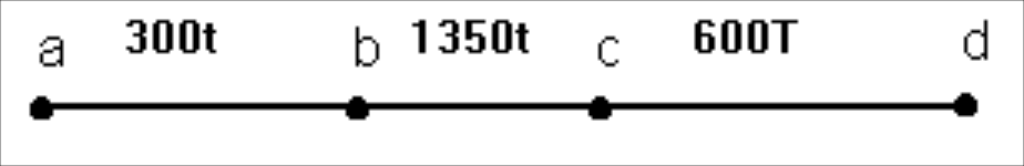
\includegraphics[width=7cm]{f3_1.png}}
\caption{\label{f3_1} Simple network of waterways}
\end{figure}

This network consists of 4 nodes and 3 links.  The links represent waterways
that can support ships of 300, 1350 and 600 tons respectively.

To get from node a to node d, the least expensive route may imply a transshippment
of the goods at node b to a ship of 1000 or 1350 tons, and transferring the goods
to a ship of 600 tons at node c.

Another possibility is to start using ships of 600 tons at node b and keep using
these to get to d.

Finally, an entire trip with ships of 300 tons would also be possible.

Although this network is a very simple one, it clearly reflects the problem of
the modal choice.

The basic idea of the proposed method is to create a virtual network, starting
from a real network.  In the virtual network all the weights, whether linked to
links or to nodes, will be assigned to links.  The notation used for the
identification codes of the nodes in this virtual network, makes it possible to
immediately know the type of cost that has to be connected to each link.  The virtual network derived from the real network presented above is represented in
figure \ref{f3_2}.


\begin{figure}[htbp]
\centerline{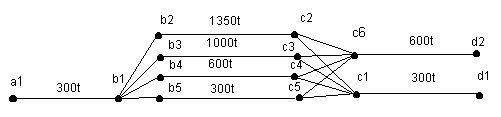
\includegraphics[width=12cm]{f3_2.png}}
\caption{\label{f3_2} Corresponding virtual network}
\end{figure}


The solution implies the creation of a new set of nodes b1-b5, c1-c5, d1-d2 and a new
set of links linking these new nodes.

In a first stage all the existing real links will be split into virtual links
according to the possible means of transportation that can be used :


\begin{itemize}
\item The link (a,b) has not been split because no other ships can pass through a
canal that can only support ships of 300 tons.
\item The link (b,c) has been split into four parts.  A canal of 1350 tons can indeed
accept ships of 300, 600, 1000 and 1350 tons pass through
\item The link (c,d) has been split into two parts, since it is possible to have
ships of 300 and 600 tons pass through the canal.
\end{itemize}


The number of real links has now more than doubled, but they still need to be connected
by means of other virtual links.  These correspond to the transshippment operations.

The real node b, for instance, is represented in the virtual network by four
virtual nodes and by four virtual links.  On these links the costs of
transshippment from a ship of 300 tons to ships of 600, 1000 and 1350 tons can be
assigned.  There is also a virtual link representing the passage from a segment
of 300 tons to another segment of 300 tons.  The weight of that link is zero; it
corresponds to the simple transit of the ship through the (real) node b, without
transshippment operations.

The same mechanism is used for the real node c.  All modal combinations are also
included in the form of virtual links and nodes.  Two links without weight have
been created for ships of 600 and 300 tons 'simple transit'.

In this way, the multi-modal network is represented by a mono-modal network on
which each link has a unique weight representing either the cost of
transportation over a certain distance, either the cost of a possible transshipment.
When a cost is assigned to each link, the cheapest path can be
computed by means of an algorithm such as the algorithm of Johnson.  The
resulting solution is an exact solution, taking all the possible choices into
account and not an heuristic leading to an approximate solution.


\section{Systematic development}

The concept of the virtual network now remains to be developed and the algorithm
for generating a virtual network starting from a real network, must be
written.  In order to make the following pages easier to read, the different
stages of the development of the algorithm will be illustrated by a simple
example of a network.



\subsection{General method}\label{General method}


Given the real network G = [X,U] of figure  \ref{f3_3}. This network is composed
of 4 nodes (\#X = N = 4) a, b, c and d and of 5 links (\#U = M = 5) numbered from 1
to 5.


\begin{figure}[htbp]
\centerline{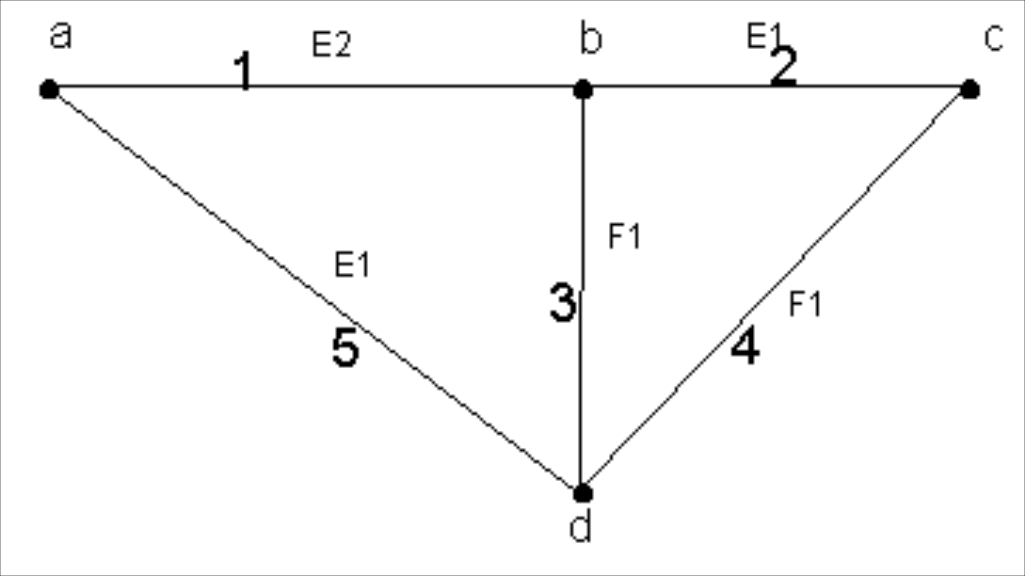
\includegraphics[width=8cm]{f3_3.png}}
\caption{\label{f3_3} Multi-modal network}
\end{figure}

Two modes of transportation are present on the network : the waterways 
\underline{W} and the railways \underline{T}. For the waterways, there are canals (E1
and E2) supporting different sizes of ships, meaning canals of 300 and of 600
tons.  On the links of type E2 it is possible to have ships of the types E1 and
E2.  There is only one type of train, F1 (diesel-powered).  It is important
to use a coherent notation for the means of transportation.  For instance, if a
link supports convoys of type E4, it has to be able to have convoys of the types
E1, E2 and E3.  For this reason the diesel-powered train is indicated by F1
and the electric train by F2, because diesel-powered trains can also
make use of electrified lines, whereas the opposite is impossible.


The table \ref{tab3_1} represents the network :

\begin{table}[htbp]
\begin{center}
\begin{tabular}{cccc}
\hline
Link number & Node 1 & Node 2 & Type of route\\
\hline
1 & a & b & E2\\

2 & b & c & E1\\

3 & b & d & F1\\

4 & d & c & F1\\

5 & a & d & F1\\
\hline
\end{tabular}
\caption{\label{tab3_1} Notation of the real network}
\end{center}
\end{table}


The first stage of the method for creating a virtual network is to examine the
set of links U and to create ($\rightarrow$) for each real link j $\in$ U as
many virtual links $\bar u_j^{tm}$ as there are possible means of transportation
connected to the transportation mode t on that link :

$$\forall _{j\in U} \forall _m u_j \rightarrow \bar u_j^{tm}$$


Each virtual link $\bar u_j^{tm}$ has two virtual end-nodes $\bar x_o^{jtm}$ and
$\bar x_d^{jtm}$ to which an identifier has been assigned, coded in four parts
as follows :


\begin{itemize}

\item  The identification code of the real node i from which the virtual node
is generated,

\item  The identification code of the real link j that has been multiplied (when
several means of transportation are possible on that link),

\item  The identification code of the mode of transportation t on the real link j,

\item  The identification code of the means of transportation m that is possible
on the new virtual link that is generated from the real link j.
\end{itemize}


A virtual node therefore can be identified by $\bar x_i^{jtm}$.

Since each real link has an origin o and a destination d, a real link will
generate the virtual links $\bar u_j^{tm}=(\bar x_o^{jtm},\bar x_o^{jtm})$ (see
table \ref{tab3_2}).


\begin{table}[htbp]
\begin{center}
\begin{tabular}{ccc}
\hline
Real links & Origin of virtual links & Destination of virtual links \\

\hline
1 & a1E2 & b1E2\\

  & a1E1 & b1E1\\

2 & b2E1 & c2E1\\

3 & b3R1 & d3R1\\

4 & d4R1 & c4R1\\

5 & a5E1 & d5E1\\
\hline
\end{tabular}
\caption{\label{tab3_2} Moving links}
\end{center}
\end{table}

\begin{figure}[htbp]
\centerline{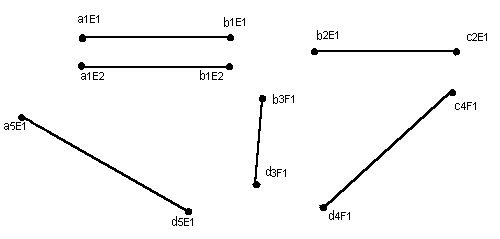
\includegraphics[width=12cm]{f3_4.png}}
\caption{\label{f3_4} Separation of the transport means}
\end{figure}


Starting from this first result (figure \ref{f3_4}), all the links representing
possible transshipments have to be generated.  This operation applies to all
real nodes. In the first phase, all real nodes have been replaced by a set of
virtual nodes.

$$\forall_{i \in X}, X_j \rightarrow \bigcup \bar x_i^{jtm} $$

All virtual nodes referring to the same real node have to be interlinked so as
to represent the set of possible transshipments \footnote {Obviously, it is not
because two links are connected that a transshipment is possible at the connexion.  This case will be discussed later.}. 


$$\forall_k \forall_{k, k\neq l}\rightarrow (\bar x_i^{ktm}, \bar x_i^{lt'm'})$$

For the real node b (figure \ref{f3_5}) this gives the figure \ref{tab3_3} :

\begin{table}[htbp]
\begin{center}
\begin{tabular}{ccc}
\hline
Real node & Origin of virtual links & Destination of virtual links \\

\hline
b & b1E1 & b1E2\\

  & b1E1 & b2E1\\

  & b1E2 & b2E1\\

  & b1E1 & b3R1\\

  & b1E2 & b3R1\\

  & b2E1 & b3R1\\

\hline
\end{tabular}
\caption{\label{tab3_3} Transshipment virtual links}
\end{center}
\end{table}

\begin{figure}[htbp]
\centerline{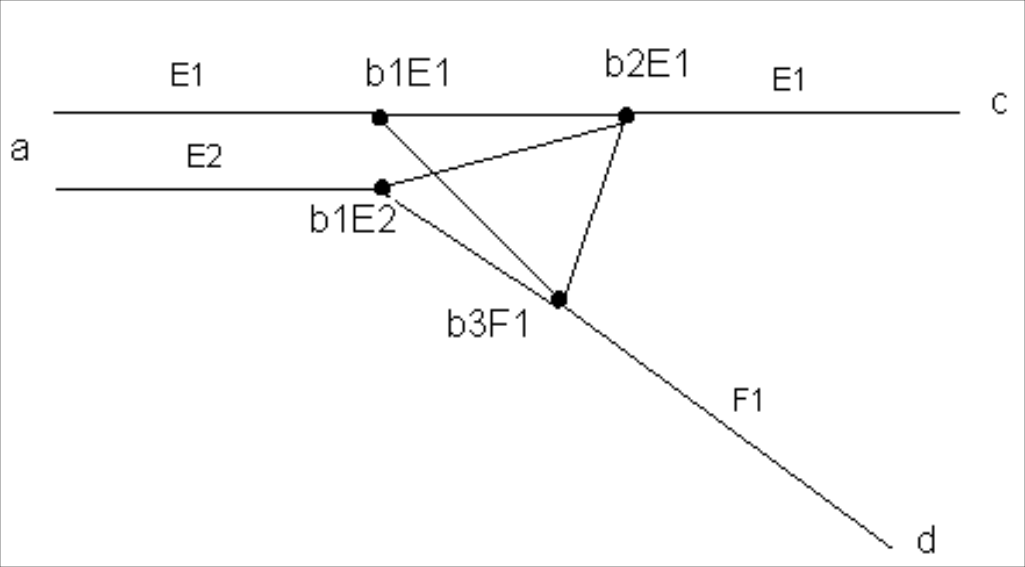
\includegraphics[width=8cm]{f3_5.png}}
\caption{\label{f3_5} Transshipments}
\end{figure}



At this stage there are two types of virtual links :

\begin{itemize}
\item The virtual links representing a distance that has to be covered.
These links represent the links of the real network, possibly multiplied if
there are several possible means of transportation.  Such a link has two virtual
end-nodes originating from two different real nodes.
\item The other virtual links represent all the possible transshipments.
Each virtual node is interlinked with all the other virtual nodes of which the
identification code refers to the same real node, excluding, however, the nodes
generated by the same real link.
\end{itemize}


The last two columns of table \ref{tab3_4} show the costs to be computed on each
virtual link.  In the case of a link that is generated directly from the real
network, it concerns a transfer between two nodes and the weight is a function
of the covered distance.  'Simple transit' costs are represented by a zero in the 'transshipment' column \footnote {In certain cases the cost
is not really zero since this type of links can also serve to represent a cost
linked, for instance, to the passage of a border or to the toll on a motorway.}.
The costs of the type "E2$\rightarrow$E1" represent the costs linked to a
transshipment, in this case the transfer from ships of 600 tons to ships of 300
tons.  There cannot be a cost in the columns "transshipment" and "shipping" at
the same time.


\begin{table}[htbp]
\begin{center}
\begin{tabular}{cccc}
\hline
Origin & Destination & Transshipment cost & Shipping cost\\
\hline
a1E1 & b1E1 & -                   & Cost = $f(distance)$\\

a1E2 & b1E2 & -                   & Cost = $f(distance)$\\

b1E1 & b2E1 & 0 & -\\ 

b1E2 & b1E1 & E2$ \rightarrow$ E1 & -\\

b1E2 & b2E1 & E2$ \rightarrow$ E1 & -\\

b1E1 & b3R1 & E1$ \rightarrow$ R1 & -\\ 

b1E2 & b3R1 & E2$ \rightarrow$ R1 & -

\\b2E1 & b3R1 & E1$ \rightarrow$ R1 & -\\ 

b2E1 & c2E1 & - & Cost = $f(distance)$\\

b3R1 & d3R1 & -                   & Cost = $f(distance)$\\
\hline
\end{tabular}
\caption{\label{tab3_4} Possible operations around the real node b}
\end{center}
\end{table}


If the same operation is repeated for all real nodes, the virtual network looks as the network represented by figure \ref{f3_6}.


\begin{figure}[htbp]
\centerline{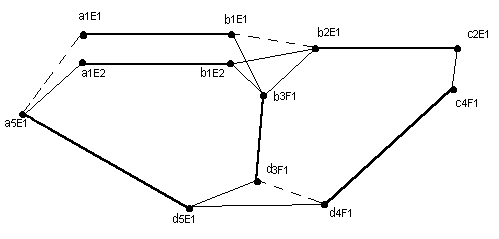
\includegraphics[width=12cm]{f3_6.png}}
\caption{\label{f3_6} Partial virtual network}
\end{figure}

In this network, the boldfaced links represent the links of the real network,
possibly split up.  The links indicated by a dotted line represent the (simple transit( virtual
links.  The transshipments, finally, are indicated by a thin
continuous line.

This method can be transcripted into an algorithm (figure \ref{algo1}), in which the symbol \# is used for the concatenation of the identification code.


\begin{center}
\begin{figure}[htbp]
\center
\fbox{
\begin{minipage}{20cm}
\begin{tabbing}
xxxxx\=xxxxx\=xxxxx\=xxxxx\=xxxxx\=xxxxx\=xxxxx\=xxxxx\=xxxxx\=xxxxx\=\kill
\bf {DEFINE} \\
tab1, tab2: arrays of virtual nodes \\ t1, t2 : indexes in these arrays\\
\\

\bf {BEGIN}\\
t1 $\leftarrow$ 1\\
\bf {FOR} j = 1 $\rightarrow$ mode $\leftarrow$ \it { transport mode on link j}\\
\> k $\leftarrow$ \it {number of transport means on link j}\\
\> \bf {FOR} l = 1 $\rightarrow$ k\\
\> \>  n1 $\leftarrow$\it {start node of link j}\\
\> \> n2 $\leftarrow$\it {end node of link j}\\
\> \> node1 $\leftarrow$ n1\#j\#mode\#k\\
\> \>  node2 $\leftarrow$ n2\#j\#mode\#k\\
\> \>  \it { Save link(node1, node2)}\\
\> \> tab[t1] $\leftarrow$ node1\\
\> \>  tab[t+1] $\leftarrow$ node2\\
\> \> t1 $\leftarrow$ t1 + 2\\
\>  \bf {END FOR} i\\
\bf {END FOR} j\\
\\
\bf {FOR} k = 1 $\rightarrow$ N\\
\> tab2[ ] $\leftarrow$ \it{part of tab1[ ] generated from node k}\\
\> t2 $\leftarrow$ \it {size of tab2[ ]}\\
\> \bf{FOR}  i = 1 $\rightarrow$ t2\\
\> \> \bf{FOR} j = i+1 $\rightarrow$ t2\\
\> \> \> \it{Save link (tab2[i], tab2[j])}\\
\> \> \bf{END FOR} j\\
\> \bf {END FOR} i\\
\bf {END FOR} k\\
\bf {END}\\
\end{tabbing}
\end{minipage}
}
\caption{\label{algo1} Basic algorithm}
\end{figure}
\end{center}




\subsection{The entry-nodes}


One problem remains unsolved : although it is possible to travel within the
virtual network, it is not possible to enter it or to leave it !  The final
user wants to find a travel route between the real nodes a and b and not between
the virtual nodes axxx and bxxx.  Moreover, there is a cost linked to entering
and leaving the network since the goods have to be loaded and unloaded.

The virtual links and nodes again offer a solution.  In the example of node b,
for instance, it is sufficient to create a new virtual node b000 and to link it
to all other virtual nodes generated for that real node.  All the new links
represent the costs of loading and unloading the goods.


$$x_i \rightarrow \bar x_i^{000}$$

$$\forall_i \forall_{ktm} \rightarrow (\bar x_i^{ktm}, \bar x_i^{000})$$



This lead, for the node b, to table \ref{tab3_5} and figure \ref{f3_7}:


\begin{figure}[htbp]
\centerline{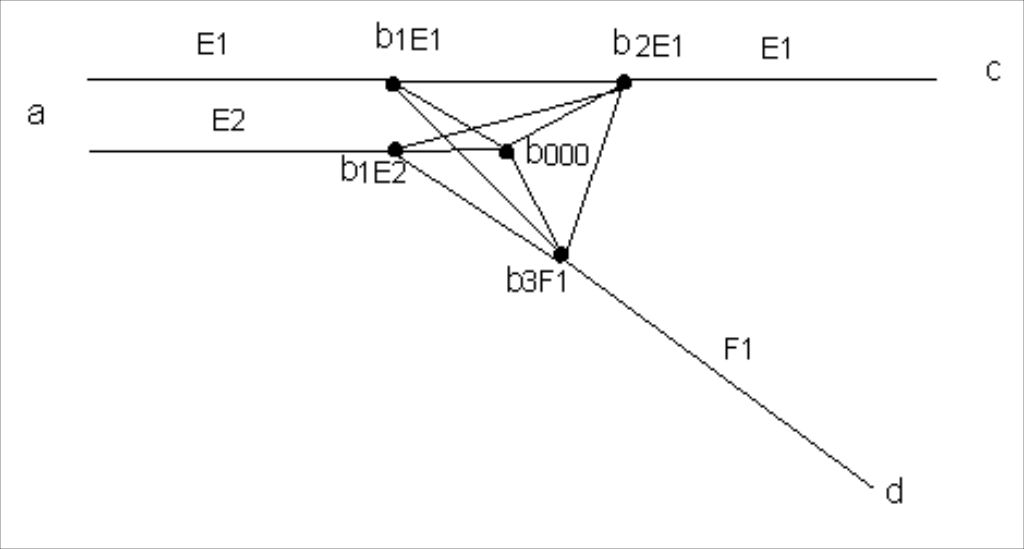
\includegraphics[width=12cm]{f3_7.png}}
\caption{\label{f3_7} Loadings/Unloadings in a virtual network}
\end{figure}

\begin{table}[htbp]
\begin{center}
\begin{tabular}{ccc}
\hline
Origin & Destination & Cost\\
\hline
b000 & b1E1 & 0 $\rightarrow$ E1\\

b000 & b1E2 & 0 $\rightarrow$ E2\\

b000 & b2E1 & 0 $\rightarrow$ E1\\

b000 & b3R1 & 0 $\rightarrow$ R1\\
\hline
\end{tabular}
\caption{\label{tab3_5} Costs on (un)loading virtual links}
\end{center}
\end{table}

In table \ref{tab3_5}, the cost represents the initial loading of the goods or their final unloading.

The algorithm shown above has to be modified to take these new virtual
nodes and links into account (see figure \ref{algo2}).


\begin{center}
\begin{figure}[htbp]
\center
\fbox{
\begin{minipage}{20cm}
\begin{tabbing}
xxxxx\=xxxxx\=xxxxx\=xxxxx\=xxxxx\=xxxxx\=xxxxx\=xxxxx\=xxxxx\=xxxxx\=\kill
\bf {DEFINE} \\
tab1, tab2: arrays of virtual nodes \\ t1, t2: indexes in these arrays\\
\\

\bf {BEGIN}\\
t1 $\leftarrow$ 1\\
\bf {FOR} j = 1 $\rightarrow$ mode $\leftarrow$ \it{transport mode on link j}\\
\> k $\leftarrow$ \it {number of transport means on link j}\\
\> \bf {FOR} l = 1 $\rightarrow$ k\\
\> \>  n1 $\leftarrow$\it {start node of link j}\\
\> \> n2 $\leftarrow$\it {end node of link j}\\
\> \> node1 $\leftarrow$ n1\#j\#mode\#k\\
\> \>  node2 $\leftarrow$ n2\#j\#mode\#k\\
\> \>  \it { Save link(node1, node2)}\\
\> \> tab[t1] $\leftarrow$ node1\\
\> \>  tab[t+1] $\leftarrow$ node2\\
\> \> t1 $\leftarrow$ t1 + 2\\
\>  \bf {END FOR} i\\
\bf {END FOR} j\\
\\
\bf {FOR} k = 1 $\rightarrow$ N\\
\> tab2[ ] $\leftarrow$ \it{part of tab1[ ] generated from node k}\\
\> t2 $\leftarrow$ \it {size of tab2[ ]}\\
\> \bf{FOR}  i = 1 $\rightarrow$ t2\\
\> \> \bf{FOR} j = i+1 $\rightarrow$ t2\\
\> \> \> \it{Save link(tab2[i], tab2[j])}\\
\> \> \bf{END FOR} j\\
\> \bf {END FOR} i\\
\\
\> \bf{FOR} i = 1 $\rightarrow$ t2\\
\> \> node $\leftarrow$ \it{"node" part of tab2[i]\#000}\\
\> \> \it{Save link(node, tab2[i])}\\
\> \bf{END FOR} i\\
\bf {END FOR} k\\
\bf {END}\\
\end{tabbing}
\end{minipage}
}
\caption{\label{algo2} Introduction of the (un)loading, virtual links}
\end{figure}
\end{center}




\subsection{The simple transit nodes}

At this stage, it is difficult to apply this method to a real network, as it often contains a serie of nodes that do not represent points where goods
are being loaded/unloaded.  The road network is characterized by a multitude of
crossroads that are also nodes, but where no goods are being loaded.  In the
same way the railway network contains some stations that are
exclusively reserved for the passengers and where transshipments of goods are
impossible.

For these nodes, no transshipment virtual links have to be
generated.

In the example of figure \ref{f3_8}, node b represents an intersection of a
waterway of 600 tons (E2) and another of 300 tons (E1).

\begin{figure}[htbp]
\centerline{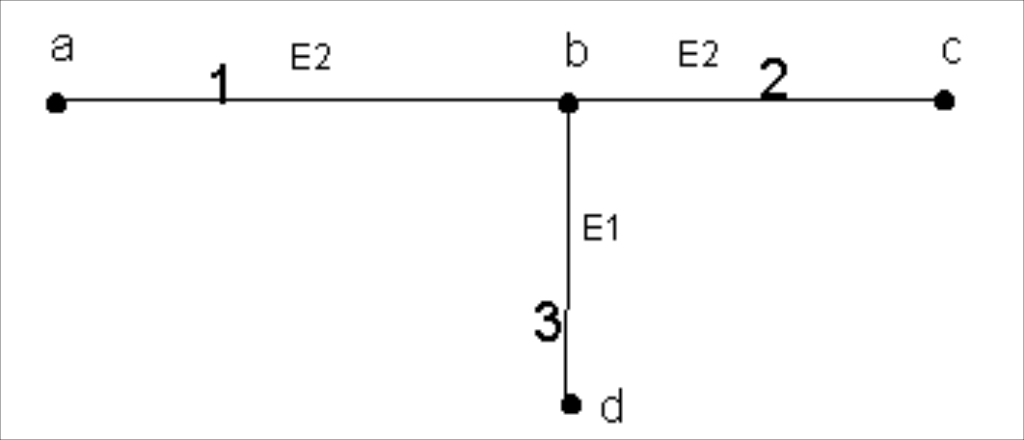
\includegraphics[width=8cm]{f3_8.png}}
\caption{\label{f3_8} Intersection of two waterways}
\end{figure}

The trunks of type E2 also support convoys of type E1.  A ship of 600 tons coming
from segment 1 can therefore continue to segment 2, but not to segment 3.

The previously explained method leads thus to the creation of the virtual nodes listed in table \ref{tab3_6}) :


\begin{table}
\begin{center}
\begin{tabular}{ccccc}
\hline
Real node & Real link & Mode & Means & Virtual node\\
\hline
b & 1 & W & 1 & b1E1\\

b & 1 & W & 2 & b1E2\\

b & 2 & W & 1 & b2E1\\

b & 2 & W & 2 & b2E2\\

b & 3 & W & 1 & b3E1\\
\hline
\end{tabular}
\caption{\label{tab3_6} Simple transit nodes}
\end{center}
\end{table}



The virtual links now need to be generated.  Again, shipping and transshipment virtual links must be generated.  This time, however, only the nodes
referring to the same combination mode-means of transportation (t = t' and m =
m') may be interlinked.  For this reason b1E2 and B2E2 will be interlinked, but
not b1E2 and b3E1 (this last combination would suggest a transshipment from a
ship of 600 tons to a ship of 300 tons and vice versa).  In other words, only
the "simple transit"virtual links are created.  Moreover, since these "transit"
nodes are not points where the network can be entered or left, the b000 node
does not need to be created, nor do the virtual links that are generated from it.


\begin{center}
If (i =  transshipment) or (t = t' and m = m') $\rightarrow
\forall_k \forall_{l} \rightarrow(\bar x_i^{ktm},
\bar x_i^{lt'm'})$\\
If i is a transshipment node $\rightarrow \forall_i
\forall_{ktm}
\rightarrow (\bar x_i^{ktm}, \bar x_i^{000})$
\end{center}

That leads to the creation of the set of links reported in table \ref{tab3_7}
(see also figure \ref{f3_9}).


\begin{table}[htbp]
\begin{center}
\begin{tabular}{cccc}
\hline

Origin & Destination & Transshipment cost & Shipping cost\\
\hline
a1E1 & b1E1 & - & $f(distance)$\\

a1E2 & b1E2 & - & $f(distance)$\\

b2E1 & c2E1 & - & $f(distance)$\\

b2E2 & c2E2 & - & $f(distance)$\\

b3E1 & d3E1 & - & $f(distance)$\\

b1E1 & b2E1 & 0 & -\\

b1E1 & b3E1 & 0 & -\\

b2E1 & b3E1 & 0 & -\\

b1E2 & b3E2 & 0 & -\\
\hline
\end{tabular}
\caption{\label{tab3_7} Virtual network at the intersection}
\end{center}
\end{table}

\begin{figure}[htbp]
\centerline{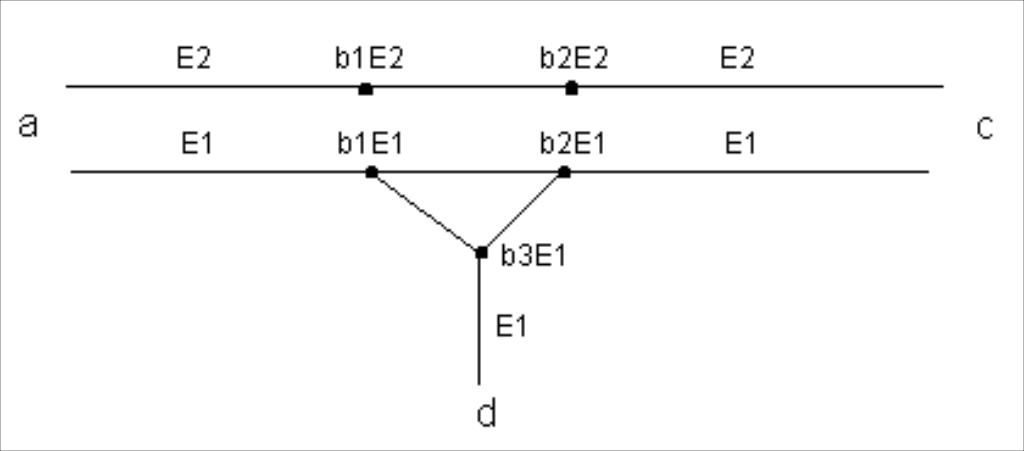
\includegraphics[width=10cm]{f3_9.png}}
\caption{\label{f3_9}  Virtual network at the intersection}
\end{figure}


The method differs according to whether the node is a place where goods are
loaded/unloaded/transshipped or simply a place of transit.  The nodes of the
graph therefore have to be marked as belonging to one of those two categories.

This differentiated treatment (see figure \ref{algo3}) has a very interesting
effect. Indeed, since the "transit" nodes generate less virtual links, the
virtual network itself will consist of clearly less links than the network
generated by the basic algorithm, an effect which will accelerate the processing
time.


\begin{center}
\begin{figure}[htbp]
\center
\fbox{
\begin{minipage}{20cm}
\begin{tabbing}
xxxxx\=xxxxx\=xxxxx\=xxxxx\=xxxxx\=xxxxx\=xxxxx\=xxxxx\=xxxxx\=xxxxx\=\kill
\bf {DEFINE} \\
tab1, tab2: arrays of virtual nodes \\ t1, t2: indexes in these arrays\\
\\

\bf {BEGIN}\\
t1 $\leftarrow$ 1\\
\bf {FOR} j = 1 $\rightarrow$ mode $\leftarrow$ \it{transport mode on link j}\\
\> k $\leftarrow$ \it {number of transport means on link j}\\
\> \bf {FOR} l = 1 $\rightarrow$ k\\
\> \>  n1 $\leftarrow$\it {start node of link j}\\
\> \> n2 $\leftarrow$\it {end node of link j}\\
\> \> node1 $\leftarrow$ n1\#j\#mode\#k\\
\> \>  node2 $\leftarrow$ n2\#j\#mode\#k\\
\> \>  \it {Save link(node1, node2)}\\
\> \> tab[t1] $\leftarrow$ node1\\
\> \>  tab[t+1] $\leftarrow$ node2\\
\> \> t1 $\leftarrow$ t1 + 2\\
\>  \bf {END FOR} i\\
\bf {END FOR} j\\
\\
\bf {FOR} k = 1 $\rightarrow$ N\\
\> tab2[ ] $\leftarrow$ \it{part of tab1[ ] generated from node k}\\
\> t2 $\leftarrow$ \it {size of tab2[ ]}\\
\> \bf{FOR}  i = 1 $\rightarrow$ t2\\
\> \> \bf{FOR} j = i+1 $\rightarrow$ t2\\
\> \> \> \bf{IF} \it{not a transshipment node}\\
\> \> \> \> \bf{AND} \it{"mode" part of tab2[i] = "mode" part of tab2[j]}\\
\> \> \> \> \bf{AND} \it{"means" part of tab2[i] = "means" part of tab2[j])}\\
\> \> \> \bf{OR} \it{transshipment node}\\
\> \> \> \> \> \bf{THEN} \it {Save link(tab2[i], tab2[j])}\\
\> \> \> \bf{END IF}\\
\> \> \bf{END FOR} j\\
\> \bf{END FOR} i\\
\\
\> \bf{FOR} i = 1 $\rightarrow$ t2\\
\> \> \bf{IF} \it{transshipment node} \bf{THEN}\\
\> \> \> node $\leftarrow$ \it{''node'' part of tab2[i]\#000}\\
\> \> \> \it{Save link(node, tab2[i])}\\
\> \> \bf{END IF}\\
\> \bf{END FOR} i\\
\bf {END FOR} k\\
\bf {END}\\
\end{tabbing}
\end{minipage}
}
\caption{\label{algo3} Introduction of the "simples transit virtual links"}
\end{figure}
\end{center}



\subsection{Orientation of the virtual network}


The method hereby proposed leads to the generation of a non oriented virtual
network.  Since each link has to be balanced by a unique weight (a cost), the
use of a non oriented graph creates the problem of the equivalence of weights
when there are transfers from origin to destination or from destination to
origin.

Such an equivalence is to strong hypothesis to be applied to a freight transportation network.  Certain
costs are a function of the direction on the link.  This is, for instance, the
case for loadings and unloadings : experience shows that it often
takes more time to unload than to load a vehicle.

In practice, the algorithm of the virtual network will generate oriented links,
which makes it possible to assign different costs according to the direction of
the virtual link. In order to generate only one (oriented) arrow between two virtual nodes (to avoid unwanted turns during the cheapest path calculation), all the nodes are ``doubled'' by giving them a positive and a negative sign. 

Using the notation used in section \ref{General method}, the virtual network generated around node b and illustrated by figure \ref{f3_7} can be represented as in figure \ref{f3_7b}.

\begin{figure}[htbp]
\centerline{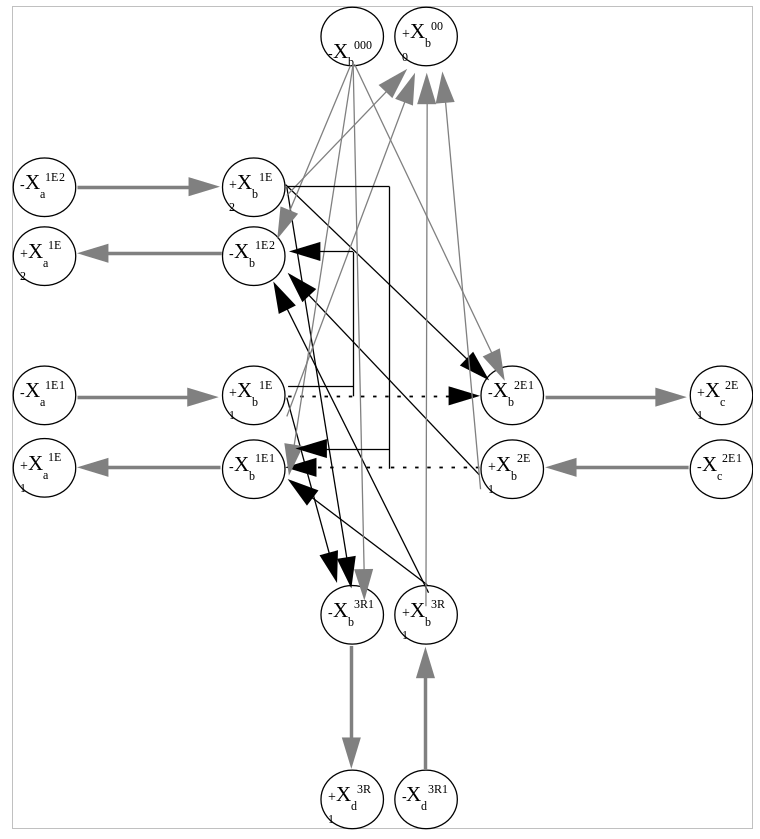
\includegraphics[width=10cm]{f3_7b.png}}
\caption{\label{f3_7b} Oriented virtual network}
\end{figure}


\subsection{Additional control on the generation of the virtual network}


The virtual network, as it has been defined for the moment, is the result of an
automatic procedure.  This way of proceeding, however, implies certain
restrictions, because some transshipment possibilities are generated
automatically whereas these movements are not possible on the real network.
This is, for instance, the case with private ports on inland waterways.  A
particular company may be authorised to load and unload goods there, but this
port does not serve as a public place of transshipment.  Therefore it is
important to be able to control the generation of the virtual network.

This check becomes possible if exclusions lists are kept for the different
nodes of the real network.  In practice it must be possible to define, for each
node of the network, the list of handling operations which would be generated
automatically but which are not possible in reality because of the physical
characteristics of the network at that location.  The generation procedure of
the virtual network is consequently adjusted, since it consults these lists of
exclusions to know whether or not a virtual link can be created.

The final algorithm is is presented in figure \ref{algo4}.

\begin{center}
\begin{figure}[htbp]
\center
\fbox{
\begin{minipage}{20cm}
\begin{tabbing}
xxxxx\=xxxxx\=xxxxx\=xxxxx\=xxxxx\=xxxxx\=xxxxx\=xxxxx\=xxxxx\=xxxxx\=\kill
\bf {DEFINE} \\
tab1, tab2: arrays of virtual nodes \\ t1, t2: indexes in these arrays\\
\\

\bf {BEGIN}\\
t1 $\leftarrow$ 1\\
\bf {FOR} j = 1 $\rightarrow$ mode $\leftarrow$ \it{transport mode on link j}\\
\> k $\leftarrow$ \it {number of transport means on link j}\\
\> \bf {FOR} l = 1 $\rightarrow$ k\\
\> \>  n1 $\leftarrow$\it {start of link j}\\
\> \> node1 $\leftarrow$ +\#n1\#j\#mode\#k and node2 $\leftarrow$ -\#n2\#j\#mode\#k\\
\> \>  \it {Save link(node1, node2)}\\
\> \> tab[t1] $\leftarrow$ node1; tab[t+1] $\leftarrow$ node2\\
\> \> t1 $\leftarrow$ t1 + 2\\
\> \> node1 $\leftarrow$ -\#n1\#j\#mode\#k and node2 $\leftarrow$ +\#n2\#j\#mode\#k\\
\> \>  \it {Save link(node2, node1)}\\
\> \> tab[t1] $\leftarrow$ node1; tab[t+1] $\leftarrow$ node2\\
\> \> t1 $\leftarrow$ t1 + 2\\
\>  \bf {END FOR} i\\
\bf {END FOR} j\\
\\
\bf {FOR} k = 1 $\rightarrow$ N\\
\> tab2[ ] $\leftarrow$ \it{ part of tab1[ ] generated from node k}\\
\> t2 $\leftarrow$ \it {size of tab2[ ]}\\
\> \bf{FOR}  i = 1 $\rightarrow$ t2\\
\> \> \bf {FOR} j = i+1 $\rightarrow$ t2\\
\> \> \> \bf{IF} \it{not a transshipment node}\\
\> \> \> \> \bf{AND} \it{"mode" part of tab2[i] = "mode" part of tab2[j]}\\
\> \> \> \> \bf{AND} \it{"means" part of tab2[i] = "means" part of tab2[j]}\\
\> \> \> \bf{OR} \it{transshipment node}\\
\> \> \> \> \> \bf{THEN IF} \it {non excluded transfer}\\
\> \> \> \> \> \> \bf{IF} \it{``node'' part of tab2[i] > 0}\\ 
\> \> \> \> \> \> \> \bf{THEN} {Save link(tab2[i], tab2[j])}\\
\> \> \> \> \> \> \> \bf{ELSE} {Save link(tab2[j], tab2[i])}\\
\> \> \> \> \> \> \bf{END IF}\\
\> \> \> \bf{END IF}\\
\> \> \bf{END FOR} j\\
\> \bf {END FOR} i\\
\\
\> \bf{FOR} i = 1 $\rightarrow$ t2\\
\> \> \bf{IF} \it{transshipment node} \bf{AND} \it{non excluded transfer} \bf{THEN}\\
\> \> \> node $\leftarrow$ -\#\it{"node" part of tab2[i]\#000}; \it{Save link(node, tab2[i])}\\
\> \> \> node $\leftarrow$ +\#\it{"node" part of tab2[i]\#000}; \it{Save link(tab2[i], node)}\\
\> \> \bf{END IF}\\
\> \bf{END FOR} i\\
\bf {END FOR} k\\
\bf {END}
\end{tabbing}
\end{minipage}
.}
\caption{\label{algo4} Algorithm of generation of a virtual network}
\end{figure}
\end{center}




\section{Assignment of the costs on the virtual links}


The virtual network makes use of four types of distinct costs : loading/unloading,
transshipping, moving and simple transit.  The type of cost to be assigned to
each virtual link can be automatically deducted from the notation used for the
two virtual end-nodes of the link.

For readability reasons, the notation used up to here has been a
notation of the type "b1E1".  It is clear that this type of notation cannot be
used in practice.  NODUS will therefore use a 10 digits integer to represent
the number of the real node, another 10 digits integer for the number of the
real link,  two digits to represent the transportation mode and two digits to
refer to the means of transportation.

As mentioned above, the virtual node is indicated in the following way (see also
table \ref{tab3_8}) :


\begin{enumerate}
\item \underline{Moving (\textbf{``mv''})}: the numbers of the real nodes are different in the two virtual nodes codes (case 1). Always from a - to a + sign.
\item \underline{Simple transit (\textbf{``tr''})}: the number of the real links vary whereas the mode and
the means of transportation have remained the same (case 2). Always from a + to a - sign.
\item \underline{Transshipment (\textbf{``tp''})}: the mode and/or means of transportation vary (case 3). Always from a + to a - sign.
\item \underline{Loading (\textbf{``ld''})/unloading (\textbf{``ul''})}: one of the two real links is "0"
(cases 4a and 4b). Always from a - to a - sign for loading and from a + to a + sign for unloading.
\end{enumerate}



\begin{table}[htbp]
\begin{center}
\begin{tabular}{crcccrccc}
\hline

Case & Node1 & Link1 & Mode1 & Means1 & Node2 & Link2 & Mode2 & Means2\\
\hline
1 & -1000 & 1000 & 1 & 1 & +1001 & 1000 & 1 & 1\\

2 & +1000 & 1000 & 1 & 1 & -1000 & 1001 & 1 & 1\\

3 & +1000 & 1000 & 1 & 1 & -1000 & 1001 & 1 & 2\\

$4_a$ & -1000 & 0 & 0 & 0 & -1000 & 1001 & 1 & 1\\

$4_b$ & +1000 & 1001 & 1 & 1 & +1000 & 0 & 0 & 0\\
\hline
\end{tabular}
\caption{\label{tab3_8} Codification of the virtual links in NODUS}
\end{center}
\end{table}


Different costs correspond to these different cases.  In the following
chapter, a general methodological framework will be provided for the development
of specific cost functions for each application.




\section{Concluding comments}


The virtual network (and NODUS, the software that implements it can be presented as :


\begin{itemize}
\item An exhaustive representation of all possible movements and operations on a
multi-modal transportation network.
\item A systematic way to generate of the elements composing the network
through an automatic procedure.
\item A general representation of a network, adapted to the realisation of a wide
range of different applications.
\item A systematic and codified notation of the elements of the network, allowing to
know the nature of the costs to be assigned to the different links.  This same
notation, based on numbers of virtual nodes coded in four parts, contains all
the necessary information on the modes and means of transportation used.  This
information can be used,  after an assignment on the network, to retrace
the modes and means of transportation that have effectively been used on the
different links composing the route.  This is an important characteristic and a valuable
aspect of the concept of the virtual network.
\end{itemize}




\chapter{Considérations générales sur les coûts}

Having briefly presented the theoretical concepts on which NODUS is based, the
different costs that can be assigned to the links of the virtual network remain to be analysed.
Unfortunately, and in spite of the existence of several network models,
the literature presents very few specific cost functions.  On the
following pages, cost elements already published will be discussed and commented
, in order to provide a general and concrete methodological framework,
applicable to the virtual network.

Economic analyses based on a network model are only significant if the
weights used on the different links of the network are credible.  These
weights can take different forms.  They can concern prices, costs, time
limits,... In order to be able to express these different forms of weights as
monetary values, the concept of "generalised cost" is often used, a basic
formulation of which was presented by Kresge and Roberts \footnote{Kresge, D.T.
and Roberts, P.O.,1971, "Techniques of Transportation Planning: Systems Analysis
and Simulation Models", Brooking Institution, Washington DC. A more depth discussion about generalised cost functions can be founded in Wilson A.G. and Bennet R.J., 1985, "Mathematical Methods in
Human Geography and Planning", John Wiley \& Sons, N-Y.} :

$$C_{ij}=f_{ij}+b_1s_{ij}+b_2\sigma s_{ij}+b_3w_{ij}+b_4p_{ij}$$

where:
\begin{itemize}
\item $f_{ij}$: direct costs supported by the operator between the nodes i and j
\item $s_{ij}$: travelling time between i and j
\item $\sigma s_{ij}$: variability of the travelling time
\item $w_{ij}$: waiting time before the actual transportation
\item $p_{ij}$: probability of having the shipment damaged or lost
\end{itemize}


In this formulation, the coefficients $b_n$ that balance the different
components of the function are generally proportional to the value of the
transported goods. After the example of the approach of Baumol and Vinod,
presented in an earlier chapter, the generalized cost offers the possibility to
assign a cost to all the variables influencing the traffic on a network.  This
way, a shipment expressed in kilometres or a waiting time expressed in hours can
be summed because expressed as monetary values.  The uncertain terms in those
formulations can, however, not be directly assigned on the network, except when
they are incorporated as average values.

The virtual network requires the development of four types of cost functions. As
mentioned above, the type of function is known through the notation used for the
virtual nodes. A concrete illustration is presented in table
\ref{tab4_1}.

\begin{itemize}
  \item Moving (\textbf{``mv''}): The identification numbers of the real nodes vary.
  \item Simple transit (\textbf{``tr''}): The identification numbers of the real links vary
whereas the mode and the means of transportation have remained the same.
  \item Transshipment (\textbf{``tp''}): The identification numbers of the real links vary,
as well as the mode and/or means of transportation.
  \item Loading (\textbf{``ld''}) / unloading (\textbf{``ul''}): One of the two identification numbers of the real
links is "0".
\end{itemize}



\begin{table}[htbp]
\begin{center}
\begin{tabular}{crcccrccc}
\hline


Case &Node1 &Link1 &Mode1 &Means1 &Node2 &Link2 &Mode2 &Means2\\
\hline
1 &-1000 &1000  &1 &01 &+1001 &1000 &1 &1\\

2 &+1000 &1000 &1 &01 &-1000 &1001 &1 &1\\

3 &+1000 &1000 &1 &01 &-1000 &1001 &1 &2 \\

4a &-1000 &0 &0 &0 &-1000 &1001 &1 &1\\

4b &+1000 &1001 &1 &1 &+1000 &0 &0 &0\\
\hline
\end{tabular}
\caption{\label{tab4_1} Examples of notation for virtual links}
\end{center}
\end{table}

Now, the cost elements that can be used with the different cases
remain to be determined, knowing that initially and intuitively, the total cost of
transportation can be resolved in the " accountancy " way presented in figure \ref{f4_1}:

\begin{figure}[htbp]
\centerline{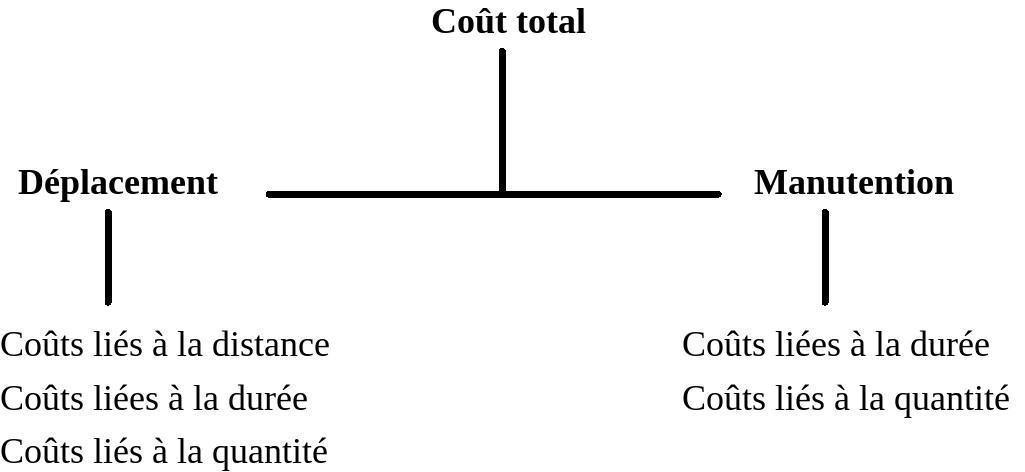
\includegraphics[width=10cm]{f4_1.png}}
\caption{\label{f4_1} Transport costs}
\end{figure}



\underline{Important remark}: It is important to keep in mind that
the functional form proposed at the end of the chapter should not be regarded as
a unique and unalterable formulation, but rather as a solution well adapted to
NODUS.  The only methodological restriction imposed by the concept of the
virtual network is the development of specific functions for the four cases
mentioned above.  The functional form of these functions can be freely chosen. Having specified this, it may be interesting to
indicate a few lines of thought, a kind of "code of good behaviour" that has to
be observed during the development of cost functions in a multi-modal
environment:



\begin{itemize}
\item Coherence of the viewpoints: a transportation can take place and be
effected by the company itself or by an independent carrier.  In the first case,
all the costs borne by the company during the transportation process have to be
analysed, whereas in the second case it is of great importance to know the
charged tariffs.  It is thus essential to adapt the same viewpoint for the
different modes of transportation taken into consideration on the network.

\item Coherence of the units: when a unit of measure is chosen (monetary units per ton, per
kilometre, per ton/kilometre,...) for a mode of transportation on a type of
virtual link, it obviously is important to use that same unit of measure for
the other modes of transportation.

\item Coherence of the variables: in the definition of the generalised costs, the same
cost factors have to be used for the different modes of transportation. If, for
instance, the duration of the trip or the financial costs are taken into
account for one mode of transportation, these same costs also have to be
introduced in the functions developed for the other modes.

\item Coherence in time: the data used in the calculations have to be time-compatible (same year of reference) for the different modes of transportation.
\end{itemize}


Having made these observations, it is possible to define a general approach of
the cost elements applicable on a virtual network.


\begin{enumerate}
\item Gathering of data while observing the principle of time-coherence
\item Development of cost functions (while observing the three other
principles of coherence)
        \begin{itemize}
        \item For all modes and means of transportation.
        \item For the four types of virtual links.
        \end{itemize}
\item Calculation of the costs on each virtual link.
\end{enumerate}

In the literature, two large categories of cost functions are
proposed.  The first one is aimed at analysing the set of costs linked to the
transportation activities.  This is an aggregated approach which, by
definition, does not apply to a network.  Unlike the first
categorie, the second type of cost functions analyses a movement from a given
origin to a given destination.  Unfortunately, this type of approach is
rather less spread, but there are certainly sufficient references to be able to
have a correct idea on the useful characteristics of transport-related costs.


The total cost of transportation consists of different parts that can be
classified in the following categories:

\begin{itemize}
\item The actual transportation: all the costs connected to the moving of
a vehicle between the points of origin and destination of the trip.

\item Inventory value: costs entailed by the storage of the goods during a certain
time span.  This part comprises real expenses such as insurances,
interest and opportunity cost (the transported goods represent a certain sum
of money, which is tied up and could have been used in another way).

\item Handling, storage: expenses linked to the manipulations of the goods beside the
actual trip.  It concerns packaging, stocking,
loading and unloading.

\item Indirect costs: costs entailed by activities subsidiary to
transport (administrative services, ...).  It is difficult to identify
these costs for a particular trip.
\end{itemize}

Besides these costs, the costs linked to congestion and the impact of the
quality of transport also need to be taken into consideration.

Congestion is indeed one of the factors influencing the cost of transportation.
It seems evident that at some moment the users of a network will encounter
congestion problems, and this has to be taken into account in the assignments.
The aim is to introduce a method able to solve the constraints linked to the
capacity of the network.

There are two fundamentally different ways to proceed:


\begin{itemize}

\item At a microscopic level, congestion leads to a slowing down of the flow and to a
choice of alternative routes to avoid traffic jams.  A solution for this
problem can be found in the network equilibrium methods that recompute the
cost functions while the flow increases.  These dynamic processes explicitly take
constraints such as the capacity of the roads or the congestion at terminals
into account.

\item At a macroscopic level, it is not always important to know whether certain
crossroads are saturated at 8 o'clock in the morning, since those crossroads are
not even introduced in the network.  However, general considerations such as the
passage through big cities or the waiting time at certain borders need to be
taken into account.  This microscopic viewpoint influences the cost functions, but
not necessarily the routes that are used.  Actually, when a large network such
as the trans-European one is digitized, the details of what is going on in a city are but rarely
dealt with.  In such a case, a digitized link can sometimes represent several
parallel routes over which the traffic will be spread over.  The cost
related to congestion can then simply be assigned to the " simple transit " virtual link in the form of a fixed cost per unit of time lost.

\end{itemize}


The quality of the transportation should be looked upon in a very broad sense
and it essentially represents the multi-products dimension of the transportation
process.  Actually, the distinction between the different products has not yet
been made, except for their inventory value.  This value, however, is not
representative since different means of transportation can be used to transport
commodities of different categories.  Imagine two types of goods of which the
weight expressed in tons is more or less the same, and which could be
transported by the same mode of transportation, but which, in practice, would be
transported by different modes of transportation and at different costs.  The
choice of the mode of transportation is thus also influenced by a certain
quality inherent to that mode and difficult to express in monetary terms.

Let us take the example of a Belgian producer exporting clothes to France.  He
chooses road transport, although it would be cheaper by
train.  A truck, however, gives him two advantages:


\begin{itemize}
\item Door to door transport;
\item Clothes are transported on hangers in the truck.
In this way, the pieces of clothing do not wrinkle.
\end{itemize}


What value should be attributed to the fact that a piece of clothing does not
wrinkle ?

Whereas factors such as time, frequence or operational safety are often found,
the concept of quality cannot that easily be introduced in a cost function.
Moreover, it is not easy to determine at what moment quality will play a role.
Is this the case while loading or while shipping ? While very interesting, this question goes 
far beyond the scope of this methodological note.

Starting from the definition of the virtual network, that requires four types of
cost functions, the table \ref{tab4_2} reflects the types of costs which
should be taken into consideration.


\begin{table}[htbp]
\begin{center}
\begin{tabular}{ll}
\hline

Type of virtual link    &Nature of the costs\\
\hline
Shipment            & Transportation\\
                    & Inventory value\\
                    & Indirects costs\\

(Un)Loading      & Handling\\
                    & Inventory value\\
                    & Indirect costs\\


Transshipment   & Handling\\
                & Storage\\
                & Inventory value\\
                & Indirect costs\\

Simple transit             & " Macroscopic " congestion \\
\hline
\end{tabular}
\caption{\label{tab4_2} Types of costs on the virtual links}
\end{center}
\end{table}



\chapter{Quelques exemples de fonctions de coût concrètes}

Les pages qui suivent vont maintenant proposer un jeu complet de fonctions de
coût pour les différents modes de transport terrestre "classiques" que sont la
route, le chemin de fer et les voies navigables. Encore une fois, ces fonctions
sont { \it une} approche possible parmi d'autres. Elles ont toutefois l'avantage
d'avoir prouvé une certaine robustesse dans une série d'applications pratiques
et publiées.



\section{Les co\^uts de d\'eplacement}

Les coûts de déplacement seront exprimés ici en unités monétaires par unité de
poins et par unité de distance parcourue (Francs par tonnes/km par exemple. Ce
sont d'ailleurs ces unités qui seront utilisées dans la suite du texte).


\subsection{Le transport}

Le coût de transport est composé de différents paramètres de nature plus
tech\-nique. Ce coût diffère en fonction des modes de transport.

\subsubsection{Voies d'eau}

\paragraph{Les péniches}

Soit:

\begin{itemize}
\item $F$ : les frais fixes annuels (annuité constante, assurances,
entretiens et salaires),
\item $u$ : le nombre d'heures de travail/année,
\item $T$ : la charge, en tonnes, de la péniche,
\item $b$ : la consommation de carburant en francs/heure,
\item $\phi$ : la vitesse de navigation moyenne.
\end{itemize}
Le coût de déplacement à la tonne et au kilomètre s'exprime par:

$$ B = \frac{F+b.u}{u.\phi . T}$$

\paragraph{Les barges}

Soit:

\begin{itemize}
\item $F_p$: les frais fixes liés au pousseur comprennent une annuité
constante, les assurances, les entretiens et les salaires,
\item $F_b$ : Les frais fixes liés aux barges comprennent uniquement une
annuité constante, les assurances et les entretiens,
\item $u$ : le nombre d'heures de travail/année,
\item $T$ : la charge, en tonnes de la barge,
\item $b$ : la consommation de carburant en francs/heure,
\item $\phi$ : la vitesse de navigation moyenne.
\end{itemize}

$$B = \frac{F_p + F_b + b.u}{u.T.\phi}$$

\subsubsection{Chemin de fer}

Comme pour les barges, les frais fixes se décomposent en $F_m$ et $F_w$, qui
représen\-tent respectivement les frais fixes liés à la motrice (annuité
constante, assurances et salaires) et ceux liés aux wagons (annuité constante,
assurances et entretien). L'entretien étant un coût fixe pour les wagons (coût
par an), il sera incorporé dans $F_w$. Par contre, les coûts d'entretien sont
variables pour la motrice et feront donc l'objet d'une formulation distincte.

Soit:

\begin{itemize}
\item $F_m$ : coût fixe lié à la motrice,
\item $F_w$ : coût fixe lié aux wagons,
\item $u$ : le nombre d'heures de travail/année,
\item $T$ : la charge, en tonnes, du train,
\item $b$ : la consommation de carburant en francs/kilomètre,
\item $\phi$ : la vitesse moyenne
\item $e$ : coût d'entretien de la motrice en francs/kilomètre
\end{itemize}


$$B=\frac{F_m+F_w}{T.u.\phi} + \frac{b+e}{T}$$
ce qui revient à:
$$B=\frac{F_m+F_w+(b+e).u.\phi}{T.u.\phi}$$

A l'instar des fonctions de coût spécifiques aux péniches et aux
barges, il s'agit ici de formes fonctionnelles très "techniques"
qui essayent de prendre en considération les paramètres les plus
pertinents liés aux coûts d'exploitation d'un train. Les valeurs
utilisées pour les calculs pratiques proviennent des statistiques
ou de comptes annuels publiés par la SNCB.

Ce type d'approche "comptable" présente parfois le danger de présenter une
sous-estimation des coûts réels, car les coûts liés à une certaine efficacité
des systèmes de transport, comme le coût salarial d'un éventuel personnel
excéden\-tai\-re, ne sont pas pris en compte.


\subsubsection{Routes}

Contrairement aux bateaux, les frais fixes ne contiennent pas les
coûts d'entretien. Pour un camion, l'entretien se fait après un
certain nombre de kilomètres.

Soit:

\begin{itemize}
\item $u$ : le nombre d'heures de travail/année,
\item $T$ : la charge, en tonnes, du camion,
\item $c$ : la consommation de carburant en francs/kilomètre,
\item $\phi$ : la vitesse moyenne,
\item $e$ : coût d'entretien en francs/kilomètre.
\end{itemize}

De ce fait

$$B=\frac{F}{T.u.\phi}+\frac{c+e}{T}$$

ce qui revient à:

$$B=\frac{F+(c+e).U.\phi}{T.u.\phi}$$


\subsection{Valeur d'inventaire}

La valeur d'inventaire représente le coût d'opportunité engendré
par l'immobili\-sation du bien transporté durant le voyage. Cette
valeur est exprimée par la charge d'intérêt sur la valeur du
chargement pour une période correspondant à la somme des durées de
voyage et de transbordement.

Soit:
\begin{itemize}
\item $V$ : valeur de la marchandise (F/tonne)
\item $R_i$ : taux d'intérêt à appliquer pour la valeur d'inventaire
\item $D$ : durée du voyage
\end{itemize}

L'expression $V.R_ii.D$ permet de connaître le coût lié à la valeur
d'inventaire durant le voyage, sous forme d'un coût d'opportunité.
Puisque la vitesse moyenne du convoi est connue, il est possible de
calculer la durée de passage sur un arc virtuel de type
"déplacement".

\subsection{Co\^uts indirects}

De par leur structure, les chemins de fer supportent de gros coûts
administratifs et autres que l'on doit, lorsque l'on se place dans
une perspective stratégique, intégrer dans le coût de transport. On
entend par "coûts administratifs et autres", l'ensemble des coûts
qui ne sont pas directement à imputer à l'activité de transport de
l'entreprise, c'est-à-dire:

\begin{itemize}
\item Services généraux,
\item Exploitation de l'infrastructure,
\item Marketing-vente,
\item Charges diverses,
\item Dotation pour risques et accidents (les compagnies de chemin de fer
prati\-quent l'auto-assurance).
\end{itemize}

Ces coûts peuvent par exemple être ramenés à une certaine somme par
tonne/ki\-lo\-mè\-tre.

\section{Les co\^uts de transbordements}

Le second type d'arcs générés dans un réseau virtuel sont les arcs
de transbor\-dement. Le coût qui doit être affecté sur ces arcs se
compose également de plusieurs aspects.

\subsection{Manutention}

Si on fait abstraction des coûts liés à l'investissement et à
l'utilisation des infrastructures, les coûts de manutention sont
fonction de la durée de cette opération. Un transbordement peut se
scinder en un déchargement et un charge\-ment dont les durées peuvent
être estimées par la formule de Deming (cfr. supra). Lorsqu'un
moyen de transport est constitué de plusieurs unités de chargement
(wagons ou barges), le temps de chargement ou de déchargement est
calculé par unité de chargement. Le temps total de chargement est
obtenu en multipliant le temps unitaire par le nombre d'unités de
chargement. Cette manière de procéder se justifie par la non
linéarité de la fonction de Deming. En effet, charger 10 wagons de
30 tonnes prend plus de temps que de charger 300 tonnes en une
fois.


\subsection{Valeur d'inventaire}

La durée de manutention, obtenue grâce à la formule de Deming, peut
être exprimée en fraction d'année. Soit $D1$ cette expression. Si
$V$ est la valeur de la marchandise et $R_i$ le taux d'intérêt à
appliquer $V.D1.Ri$ exprime la charge d'intérêt supportée pendant
le chargement et/ou le déchargement d'une tonne de marchandise de
valeur $V$.

\subsection{Co\^uts indirects}

Sous cette rubrique, seront considérés les coûts liés à
l'immobilisation des véhi\-cules lors des opérations de manutention.

\subsubsection{Voies d'eau}

\paragraph{Les péniches}

Soit:

\begin{itemize}
\item $F$: les frais fixes annuels (annuité constante, assurances,
entretiens et salaires),
\item $L$ : le temps de chargement ou de déchargement,
\item $u$ : le nombre d'heures de travail/année,
\item $T$ : la charge, en tonnes, de la péniche,
\item $n$ : le nombre de personnes qui chargent ou déchargent.
\end{itemize}

Le coût fixe, à la tonne, peut dès lors s'exprimer par:

$$A=\frac{F.\frac{L}{N}}{u.T}$$

\paragraph{Les barges}

Soit:

\begin{itemize}
\item $Fp$ : les frais fixes liés au pousseur,
\item $F_b$ : les frais fixes liés aux barges,
\item $t$ : le temps nécessaire pour former le convoi,
\item $L$ : le temps de chargement ou de déchargement,
\item $u$ : le nombre d'heures de travail/année,
\item $T$ : la charge, en tonnes, de la péniche,
\item $n$ : le nombre de personnes qui chargent ou déchargent.
\end{itemize}

Les frais fixes liés au pousseur comprennent une annuité constante,
les assurances, les entretiens et les salaires. Les frais fixes
liés aux barges comprennent uniquement une annuité constante, les
assurances et les entretiens.

$$A=\frac{F_p.t+\frac{F_b.L}{n}}{u.T}$$

\subsubsection{Chemin de fer}

Comme pour les barges, les frais fixes se décomposent en $F_m$ et
$F_w$.

\begin{itemize}
\item $L$ : le temps de chargement ou de déchargement,
\item $u$ : le nombre d'heures de travail/année,
\item $T$ : la charge, en tonnes, du train,
\item $n$ : le nombre de personnes qui chargent ou déchargent,
\item $t$ : le temps nécessaire pour former le convoi en gare de triage.
\end{itemize}

De ce fait,

$$A=\frac{F_m.t+\frac{F_w.L}{n}}{u.T}$$

\subsubsection{Routes}

Soit:

\begin{itemize}
\item $F$: frais fixes,
\item $L$ : le temps de chargement ou de déchargement,
\item $u$ : le nombre d'heures de travail/année,
\item $T$ : la charge, en tonnes, de la péniche,
\item $n$ : le nombre de personnes qui chargent ou déchargent.
\end{itemize}


$$A=\frac{F.\frac{L}{n}}{u.T}$$


\section{Les co\^uts de chargement et d\'echargement}

Ce troisième type d'arc virtuel se voit attribuer une structure de
coût très semblable à ce qui a été défini pour les transbordements.

Dans ce cas, il faut parfois tenir compte du transit par un
entrepôt.

\subsection{Manutention}

Le lecteur peut, pour ce type de coûts, se référer aux fonctions
présentées dans la partie "Coûts de transbordements".

\subsection{Magasinage}

Il est très difficile de développer une fonction de coût générale
pour l'entreposage. En effet, ce dernier varie en fonction de
différents paramètres: chaque entrepôt est différent et fonctionne
de manière différente. Pour simplifier le problème, on peut
considérer un montant fixe à la tonne, bien que cette manière de
faire soit critiquable.

\subsection{Valeur d'inventaire}

Voir "Coûts de transbordement".

\subsection{Co\^uts indirects}

Voir "Coûts de transbordement".

\section{Simple passage}

Il reste le quatrième et dernier type d'arc virtuel, celui qui
représente le "simple passage", sur lequel on peut affecter un coût
lié à la congestion, si un modèle d'équilibre n'est pas mis en
oeuvre.

D'autres coûts peuvent également être affectés aux arcs virtuels de simple
passage. C'est ainsi que les coûts induits par le passage des frontières ou ceux
engendrés par des contraintes techniques (changement d'écartement de voies,...)
peuvent être pris en considération. Ce genre de coûts est introduit dans nos
fonctions par l'intermédiaire d'un coût fixe, associé à certains noeuds du
réseau.

En effet, ces noeuds (réels) donnent naissance à des arcs
(virtuels) sur lesquels il est possible d'affecter une fonction de
coût. Une partie des ces arcs virtuels est constituée d'arcs
virtuels de simple passage entre deux arcs de même mode/moyen de
transport.  Le cas d'un passage de frontière ou d'un péage
autoroutier illustre bien l'utilisation qui peut être faite des
arcs de simple passage. En effet, un passage de frontière
n'implique pas un changement de mode/moyen de transport. Par
contre, il y a souvent des formalités administratives qui prennent
un certain temps et qui coûtent dès lors de l'argent. Ce type de
coût peut très bien être affecté à un arc virtuel de simple
passage. Ce raisonnement peut également être tenu pour prendre en
considération les coûts liés aux péages sur les autoroutes.


\end{document}
